\documentclass[a4paper,11pt]{article}

\usepackage[utf8x]{inputenc}	
\usepackage{fullpage}		
\usepackage[T1]{fontenc}				
\usepackage[english]{babel}			
%\usepackage{ulem}
\usepackage{xcolor}						
\usepackage{amsmath,amstext,amssymb,amsfonts,amsthm,mathrsfs,chemarrow,stackrel,dsfont}   % Math packages
\usepackage{graphicx} 					
\usepackage{subcaption}					
%\usepackage{cite}	
\usepackage[authoryear,sectionbib,sort]{natbib} % Bio citation format
\linespread{1.7}
\usepackage{titlesec}
\titleformat{\section}[block]{\Large\bfseries\filcenter}{\thesection}{1em}{}
\titleformat{\subsection}[block]{\Large\itshape\filcenter}{\thesubsection}{1em}{}
\titleformat{\subsubsection}[block]{\large\itshape}{\thesubsubsection}{1em}{}
\titleformat{\paragraph}[runin]{\itshape}{\theparagraph}{1em}{}[. ]\renewcommand{\refname}{Literature Cited}

\usepackage{microtype}
\usepackage{array}
\usepackage{booktabs}
\usepackage{makecell}

%%%%%% XX To be removed before submission!
\usepackage{lineno}
\usepackage{showlabels}

\usepackage[pdftex, breaklinks, colorlinks, citecolor=black, urlcolor=black, linkcolor=black]{hyperref} 
\usepackage{fourier} % FD I try to avoid the default LaTeX font for non math journals
\usepackage{FiraSans}
\usepackage{soul}

% Packages to comment out before submitting!
%\usepackage[textsize = scriptsize, backgroundcolor = white, linecolor = black]{todonotes}
%\usepackage{showlabels}

%\numberwithin{equation}{section}
%\setlength{\parindent}{0pt}
\allowdisplaybreaks[2]

\newcolumntype{P}[1]{>{\centering\arraybackslash}m{#1}}     % Table formatting
\renewcommand{\arraystretch}{1.1}                           % Table formatting

\definecolor{darkgreen}{rgb}{0.0, 0.42, 0.24}
\definecolor{darkblue}{rgb}{0.0, 0.0, 0.55}
\definecolor{change}{rgb}{0.5,0.,0.6}

%%%%%% our commenting commands
\newcommand{\florence}[1]{\textcolor{purple}{(#1)}} % Changed red to purple
\newcommand{\francois}[1]{\textcolor{blue}{(#1)}}
\newcommand{\hildegard}[1]{\textcolor{darkgreen}{(#1)}}
\newcommand{\pete}[1]{\textcolor{orange}{(#1)}}
\newcommand{\chg}[1]{\textcolor{change}{#1}}

%opening
\title{The effect of habitat choice on evolutionary rescue in subdivided populations}
\author{Peter Czuppon$^{1,2,\ast}$, Fran\c{c}ois Blanquart$^{1,3}$, Hildegard Uecker$^{4,\dag}$,\\ Florence D\'{e}barre$^{2,\dag}$}
\date{}


\begin{document}

\maketitle

\vspace{-20pt}
\noindent $^1$ Center for Interdisciplinary Research in Biology, CNRS, Coll\`ege de France, PSL Research University, Paris, France.

\noindent $^2$ Institute of Ecology and Environmental Sciences of Paris, Sorbonne Universit\'e, UPEC, CNRS, IRD, INRA, Paris, France.

\noindent $^3$ IAME, UMR 1137, INSERM, Universit\'{e} Paris Diderot, Paris, France.

\noindent $^4$ Research Group ``Stochastic evolutionary dynamics'', Department of Evolutionary Theory, Max-Planck Institute for Evolutionary Biology, Pl\"{o}n, Germany.

\noindent $\ast$ Corresponding author; e-mail: peter.czuppon@college-de-france.fr.

\noindent $^\dag$ Equal contribution.

\noindent The authors wish to be identified to the reviewers.

\bigskip

\textit{Manuscript elements}: Figures~1-6, Table~1, Supplementary Information including figures S1-S6. All figures are to print in color.

\bigskip

\textit{Keywords}: evolutionary rescue, local adaptation, source-sink dynamics, dispersal, gene flow, habitat choice, density-dependent dispersal.

\bigskip

\textit{Manuscript type}: Article. %Or e-article, note, e-note, natural history miscellany, e-natural history miscellany, comment, reply, invited symposium, or countdown to 150.

\newpage

\linenumbers{}
\modulolinenumbers[2]

\begin{abstract}
    \noindent \textbf{Abstract} Evolutionary rescue is the process by which a declining population successfully adapts genetically\footnote{\francois{remove genetically}\florence{ok to remove}} to avoid extinction. In a structured environment that deteriorates patch by patch, dispersal can substantially alter the chances of evolutionary rescue of a \linelabel{R2-1}\chg{population whose wild type is} not viable in deteriorated patches. Here, we investigate the effect of different dispersal schemes and intensities on the probability of successful establishment of a mutant population adapted to the deteriorated environment. \linelabel{R1-2}\chg{We assume that local fitness is determined by a single haploid locus\florence{ and that d}\st{. D}ispersal is genotype-dependent\st{ and linked to the adaptive trait, i.e. dispersal does not evolve by itself}\footnote{\florence{[otherwise it sounds like $m$ is changing...] [need to add that it's the bias that is changing, not the probability to emigrate]}}. In this scenario, we }find that the probability of evolutionary rescue can undergo up to three phases when increasing the rate of dispersal\footnote{\florence{since you specify ``at low disp'', ``at intermediate disp'' etc., you can remove ``when increasing the rate of dispersal'' to save words}}: (i) at low dispersal rates, the probability of establishment of a mutant population increases; (ii) at intermediate dispersal rates, the establishment probability decreases; (iii) at large dispersal rates, the population homogenizes, \florence{, which either promotes or suppresses}\footnote{\florence{old version: either promoting or suppressing}} the process of evolutionary rescue, depending on the fitness difference between the mutant and the wild type. Our results show that habitat choice\footnote{\florence{up to now, the reader does not know this is about habitat choice (``schemes'' is not precise enough}}, when compared to \chg{unbiased} dispersal, impedes successful adaptation when the mutant has the same habitat preference as the wild type, but promotes adaptation when the mutant mainly immigrates into patches where it has a growth advantage over the wild type.
\end{abstract}

%\textit{Keywords:} evolutionary rescue, local adaptation, source-sink dynamics, dispersal, gene flow, habitat choice, density-dependent dispersal

%%%%%%%%%%%%%%%%%%%%%%%%%%%%%%%%%%%%%%%%%%%%%%%%%%%%%%%%%%%%%%%%%%%
%%%%%%%%%%%%%%%%% INTRODUCTION %%%%%%%%%%%%%%%%%%%%%%%%%%%%%%%%%%%%
%%%%%%%%%%%%%%%%%%%%%%%%%%%%%%%%%%%%%%%%%%%%%%%%%%%%%%%%%%%%%%%%%%%
\newpage
\section*{Introduction}

%%%%%%%%%%%%%%%%%%%%%%%%%%%%%%%%%%%%%%%%%%%%%%%%%
% Evol rescue and empirical evidence %%%%%%%%%%%%
%%%%%%%%%%%%%%%%%%%%%%%%%%%%%%%%%%%%%%%%%%%%%%%%%
Facing current anthropogenic environmental changes such as deforestation, soil and water contamination or rising temperatures, the populations of many species are declining and might eventually go extinct \citep{bellard_2012, diniz_2019}. Pests and pathogens experience similarly strong selective pressures as a result of increased consumption of antibiotics and use of pesticides \citep{ramsayer_2013, kreiner_2018}. 
The process of genetic adaptation that saves populations from extinction is termed evolutionary rescue. This \linelabel{R1-3}\chg{process is characterized by an initial population decline (that would result in population extinction) followed by recovery due to the establishment of adapted genotypes, typically }resulting in a U-shaped demographic trajectory over time~\citep{gomulkiewicz_1995}.
In recent years, empirical examples of evolutionary rescue have accumulated \citep[as reviewed by ][]{alexander_2014,carlson_2014,bell_2017}. Evolutionary rescue \linelabel{R1-4}\chg{has been observed directly in laboratory experiments \citep[e.g.][]{bell_2009,agashe_2011,lachapelle_2012,lindsey_2013,stelkens_2014}. In wild populations demographic and genotypic data is rarely monitored at the same time impeding direct observation of evolutionary rescue. Still, it has been suggested as a mechanism that has saved a few wild populations from extinction \citep[e.g.][]{vanderwal_2012,digiallonardo_2015,gignoux_2018}.} 

%%%%%%%%%%%%%%%%%%%%%%%%%%%%%%%%%%%%%%%%%%%%%%%%%
% Evol rescue and dispersal %%%%%%%%%%%%%%%%%%%%%
%%%%%%%%%%%%%%%%%%%%%%%%%%%%%%%%%%%%%%%%%%%%%%%%%
In mathematical models, evolutionary rescue is often studied in a spatially homogeneous situation where the whole population experiences a sudden decrease in habitat quality. In this setting, a large number of theoretical results have been established, for example on the effects of recombination \citep{uecker_2015} and horizontal gene transfer \citep{tazzyman_2014}, reproduction mechanisms \citep{glemin_2013,uecker_2017}, intra- and interspecific competition \citep{osmond_2013}, predation pressure \linelabel{R1-5}\chg{\citep{yamamichi_2015}}, bottlenecks \citep{martin_2013}, different genetic pathways \citep{osmond_2019}, and the context-dependent fitness effects of mutations \citep{anciaux_2018}. \chg{In contrast to these abrupt change scenarios, evolutionary rescue can also be studied in a gradually changing environment \citep[e.g.][]{osmond_2017}}\footnote{\pete{Does anybody know other references?} \hildegard{What about Lynch et al. 1991. Adaptive and  demographic responses of plankton populations to environmental change. Limnology and Oceanography 36:1301--1312., B{\"u}rger and Lynch 1995. Evolution and extinction in a changing environment: a quantitative genetic analysis. Evolution 49:151--163 and Lande and Shannon 1996. The role of  genetic  variation  in adaptation and population persistence in a changing environment. Evolution 50:434--437? But please check; it's a long time that I read those...}}. 
In fragmented environments, habitat deterioration is not necessarily synchronized across patches: there can be a transient spatially heterogeneous environment consisting of old- and new-habitat patches until eventually the whole environment has deteriorated. If individuals that populate different patches are able to move between those, the effect of dispersal on evolutionary rescue needs to be taken into account \citep{uecker_2014, tomasini_2019}. Experiments that study the effect of dispersal on evolutionary rescue are rare but indicate that \linelabel{R1-6} dispersal can increase the likelihood of successful genetic adaptation \citep{bell_2011}. 

\linelabel{R1-1}\chg{Evolutionary rescue in a fragmented environment can be interpreted as the intermediate situation between abrupt change and gradual change: if dispersal is very low, patches are approximately isolate and thus each patch undergoes an abrupt change independent of the other patches; if the dispersal rate and the number of patches are very high, the whole environment is gradually changing since spatial structure and the contribution of a single patch are negligible.}

%%%%%%%%%%%%%%%%%%%%%%%%%%%%%%%%%%%%%%%%%%%%%%%%%
% Adaptation and dispersal %%%%%%%%%%%%%%%%%%%%%%
%%%%%%%%%%%%%%%%%%%%%%%%%%%%%%%%%%%%%%%%%%%%%%%%%
Evolutionary rescue in a situation where one patch after \linelabel{R2-2}\chg{another} deteriorates is tightly linked to the study of adaptation to a heterogeneous environment with source-sink dynamics. These describe a spatially heterogeneous environment that is constant in time where a population in unfavorable habitats can be maintained by constant immigration of the wild type. Experimental and theoretical studies have found that \linelabel{R2-3}\chg{increasing} dispersal can have a positive or a negative effect on genetic adaptation in a heterogeneous environment (see e.g. \citet{holt_1997,gomulkiewicz_1999} for positive; \citet{storfer_1998,garcia_1997,kirkpatrick_1997,fedorka_2012} for negative; and \linelabel{R1-7}\chg{\citet{kawecki_2000,ronce_2001,gallet_2018}} for both effects).
%Reason for different results: (i) demography or not (Kawecki); (ii) selection strength (Gallet), (iii) selection strength (Ronce)
\florence{suggestion: focus on discrete traits - thousands of possible papers to cite; avoid RK2001}

In theoretical studies of local adaptation and evolutionary rescue, dispersal is typically assumed to be \chg{unbiased}, i.e. dispersing individuals are distributed uniformly among patches. Only few investigations in the context of local adaptation in source-sink systems have taken into account non-\chg{uniform} dispersal patterns \citep[e.g.][]{kawecki_1995,holt_1996,kawecki_2002,amarasekare_2004}. This analytical focus on \chg{unbiased} dispersal is in stark contrast to actually observed dispersal schemes in nature \citep[][]{edelaar_2008,clobert_2009,edelaar_2012}. Here, we explore and compare the effects of several biologically motivated dispersal schemes on adaptation and evolutionary rescue.

%%%%%%%%%%%%%%%%%%%%%%%%%%%%%%%%%%%%%%%%%%%%%%%%%
% Empirical examples for non-random dispersal %%%
%%%%%%%%%%%%%%%%%%%%%%%%%%%%%%%%%%%%%%%%%%%%%%%%%
One of the best documented modes of non-\chg{uniform} dispersal is density-dependent dispersal. Density dependence can be positive or negative: either individuals prefer to settle or stay in large groups (positive density-dependence), or they choose to remain in or move to less populated regions (negative density-dependence). Density-dependent dispersal, of either form, is ubiquitously found in nature and has been reported in many species across the tree of life, including insects \citep{endriss_2019}, spiders \citep{meester2010}, amphibians \citep{gautier_2006}, birds \citep{wilson_2017}, fishes \citep{turgeon_2012}, and mammals~\citep{stoen_2006}.

Another well-established dispersal scheme is habitat choice, whereby individuals tend to immigrate into habitats they are best adapted to. This mechanism has for example been reported in lizards \citep{bestion_2015}, birds \citep{dreiss_2011,benkman_2017}, fishes \citep{bolnick_2009}, worms \citep{mathieu_2010}, and ciliates \citep{jacob_2017,jacob_2018}. 

\linelabel{R1-8}\chg{Although density-dependence or habitat choice can also affect the emigration behavior, i.e. the likelihood that an individual leaves its current location, or even the vagrant stage when the individual is in the process of dispersal \citep{bowler_2005,ronce_2007}, we ignore this here. Instead, we concentrate on \chg{non-uniform} dispersal effects of the immigration process.} \\

%%%%%%%%%%%%%%%%%%%%%%%%%%%%%%%%%%%%%%%%%%%%%%%%%
% What do we do? %%%%%%%%%%%%%%%%%%%%%%%%%%%%%%%%
%%%%%%%%%%%%%%%%%%%%%%%%%%%%%%%%%%%%%%%%%%%%%%%%%
In the following, we explicitly account for these \chg{biased} dispersal schemes in the context of genetic adaptation to a deteriorating and spatially structured environment. We model an environment that consists of various patches with one of two possible habitats: the `old' habitat, in which both \linelabel{R1-9-1}\chg{types, wild type and mutant, have a positive growth rate}, and the `new' habitat, where in the absence of immigration the wild-type population will eventually go extinct. In this framework, we study four biologically motivated dispersal patterns and compare them to the \chg{unbiased} dispersal scheme. We start by investigating their consequences for the establishment dynamics of an adapted mutant in a time-constant heterogeneous environment. 
From there, we derive an approximation for adaptation in a source-sink setting.
Using these results, we study the probability of evolutionary rescue, i.e. of adaptation in the scenario where patches, one after \chg{another}, deteriorate over time until all locations contain the new habitat. We find that dispersal bias has a direct effect on the local growth rates which in turn affect the probability of establishment and evolutionary rescue.

%%%%%%%%%%%%%%%%%%%%%%%%%%%%%%%%%%%%%%%%%%%%%%%%%%%%%%%%%%%%%%%%%%%
%%%%%%%%%%%%%%%%% MODEL %%%%%%%%%%%%%%%%%%%%%%%%%%%%%%%%%%%%%%%%%%%
%%%%%%%%%%%%%%%%%%%%%%%%%%%%%%%%%%%%%%%%%%%%%%%%%%%%%%%%%%%%%%%%%%%
\section*{Model}
%%%%%%%%%%%%%%%%%%%%%%%%%%
% General description %%%%
%%%%%%%%%%%%%%%%%%%%%%%%%%
We consider a spatially structured environment consisting of $M$ patches all connected to each other. The habitat of a patch is either in the \textit{old} or in the \textit{new} state, corresponding to habitat quality before and after environmental deterioration, respectively. The transition from the old to the new habitat is assumed to be irreversible. Patches are populated by two types of asexually reproducing, haploid individuals, either wild type or mutant. Generations are measured in discrete time steps and are non-overlapping. \linelabel{R1-9-2}\linelabel{R2-6}\chg{Wild-type and mutant individuals both have a positive growth rate} in old-habitat patches; the mutant has a lower growth rate there. In new-habitat patches, the wild type population declines locally while the mutant has a positive growth rate -- we will therefore call it a `rescue mutant'. \chg{Both habitat types, old and new, have a (potentially different) carrying capacity. At the end of a life cycle, the local population size is reduced to the carrying capacity if necessary.}

We consider a time-varying environment, such that one after \chg{another} every $\tau$ generations, the habitat of a patch deteriorates (from old to new state). Initially ($t<0$), all patches are of the old-habitat type. At time $t=0$, the first patch deteriorates. After $(M-1)\tau$ generations, all patches are of the new-habitat type. We denote the time-dependent frequency of old-habitat patches by $f_{\text{old}}$. It equals $1$ before the first environmental change takes place ($t<0$), and decreases by $1/M$ after each environmental deterioration event until it eventually hits~$0$, when all patches have undergone the environmental change. This environmental setting corresponds to the one analyzed by \citet{uecker_2014} and more recently in the special case of just two patches by \citet{tomasini_2019}.

The individuals are assumed to go through the following life-cycle: (i) Dispersal: individuals may move between patches; (ii) Reproduction: individuals reproduce within patches. \linelabel{R2-7}\chg{The number of offspring per parent is modeled by a Poisson number}; (iii) Mutation: wild-type individuals mutate to the rescue mutant type with probability $\theta$ -- back mutations from the mutant to the wild type are neglected; (iv) Regulation: the population size is, \chg{if necessary, down-regulated to the carrying capacity $K_k$ where $k$ refers to the habitat type (old or new - the two habitat types can have different carrying capacities)}. If the population size is below the carrying capacity, the regulation step is ignored. 

%%%%%%%%%%%%%%%%%%%%%%%%%%
% Old habitat dynamics %%%
%%%%%%%%%%%%%%%%%%%%%%%%%%
\subsection*{Old-habitat dynamics}
\linelabel{R1-10}We assume that in old-habitat patches, \linelabel{R1-9-3}\chg{both types have a positive growth rate such that the population in these patches is typically at carrying capacity $K_{\text{old}}$.} We denote the fecundities of the \textbf{w}ild-type and the \textbf{m}utant by $\omega_w$ and $\omega_m$, respectively. 
We impose an adaptation trade-off for the rescue mutant, i.e. the mutant is less fit than the wild type in old-habitat patches ($\omega_m<\omega_w$).
%
\linelabel{R2-9}\chg{We assume that mutation from the wild type to the mutant is tied to reproduction. The probability that an offspring of a wild-type individual is a mutant is given by $\theta$. We neglect back-mutation from mutant to wild type.} 
\linelabel{R2-8}\chg{After reproduction, if the population size exceeds the carrying capacity $K_{\text{old}}$ we randomly remove individuals from the population until the carrying capacity is reached\linelabel{AE-3}, i.e. we assume that the wild type and the mutant are competitively equivalent. The mean number of offspring of\footnote{\francois{produced by}} one mutant after reproduction and population regulation is then given by   
\begin{equation}\label{eq:sold}
     K_{\text{old}}\, \frac{\omega_m}{\omega_w \widetilde{N}^{\text{old}}_w + \omega_m}\approx K_{\text{old}}\, \frac{\omega_m}{\omega_w \widetilde{N}^{\text{old}}_w} =1 + a_{\text{old}} \, ,
\end{equation}
where the random variable $\widetilde{N}_{i}^{k}$ denotes the population sizes of type $i$ (mutant or wild-type) in patches with habitat $k$ (old or new) after the dispersal step. Additionally, we have defined the local growth rate of a single mutant, denoted by $1+a_{\text{old}}$. \linelabel{R1-11}The approximation in eq.~\eqref{eq:sold} holds if the number of mutants is much lower than the number of wild types in old-habitat patches -- a reasonable assumption since the establishment of the mutant is decided when it is still rare.}
%Then, while still rare, mutant individuals will reproduce independently of each other and their dynamics will be described by the local growth rate given in eq.~\eqref{eq:sold}. 
\chg{Compared to the wild type we assume a reduced fecundity of the mutant in the old habitat, i.e. $\omega_m<\omega_w$. Still, the local growth rate can be positive, that is, larger than one ($a_{\text{old}}>0$).} This happens when the \linelabel{R2-12}\chg{wild-type population in a single old-habitat patch after dispersal,} \linelabel{R1-13}$\widetilde{N}^{\text{old}}_w$, becomes very small. This strongly depends on the dispersal scheme and rate. \linelabel{R1-14}\chg{The population dynamics of the wild type are analyzed explicitly in Section~1 of the Supplementary Information (SI).}

%%%%%%%%%%%%%%%%%%%%%%%%%%
% New habitat dynamics %%%
%%%%%%%%%%%%%%%%%%%%%%%%%%
\subsection*{New habitat dynamics}
In the new habitat and in the absence of immigration, the wild-type population will go extinct. To account for this, we assume that the number of wild-type \linelabel{R1-15}offspring \chg{per parent} in new-habitat patches is a Poisson distributed value with parameter $(1-r)$, where $r$ measures how strongly the wild type is affected by the environmental deterioration. For $r=1$ the wild-type population becomes locally extinct in new-habitat patches after one generation.

The mutant type, in contrast, has a local growth rate larger than one and will (in expectation) grow in numbers. The number of offspring is again Poisson distributed with per-capita rate $(1+a_{\text{new}})$, the local growth rate of the mutant in new-habitat patches. 

\linelabel{R1-17}\linelabel{R2-13}\chg{In the following analysis we will assume that the mutant dynamics in new-habitat patches are density-independent. This is a valid assumption as long as the carrying capacity in these patches, $K_{\text{new}}$, is not reached. Of course, in the simulations the carrying capacity might sometimes be reached, especially for large frequencies of old-habitat patches. This assumption on density-independence also restricts our choice for the carrying capacity in the new habitat. If the carrying capacity in new-habitat patches is much smaller than in old-habitat patches, the new habitat can reach its carrying capacity merely due to immigration of wild-type individuals (even after reproduction where the wild-type population is reduced).\footnote{\francois{Rephrase, as this is not clear. What carrying capacity do you choose and whether your approximation holds or not. Maybe: `Here we examine a carrying capacity in new habitats which is half that in old habitats. If the carrying capacity were much smaller, our analytical approximation would break down.}}}


%%%%%%%%%%%%%%%%%%%%%%%%%%
% Dispersal mechanisms %%%
%%%%%%%%%%%%%%%%%%%%%%%%%%
\subsection*{Dispersal mechanisms}

We assume that dispersal is cost-free, i.e. all emigrating individuals will settle in a patch, leaving the global population size before and after dispersal unchanged. \linelabel{R1-18}\linelabel{R2-14}\chg{Note however, that our methods are in principle also applicable to a scenario where dispersal is associated with a (potentially type-dependent)\footnote{\francois{remove bracket}} cost.} We split the dispersal step into emigration and immigration. We focus on habitat choice during immigration. Individuals have a bias to immigrate into patches of a certain habitat type. The bias \chg{during} immigration \chg{for} new-habitat patches is set to \chg{zero}, without loss of generality.\footnote{\francois{I did not understand why this is needed}} The bias \chg{for immigration to} an old-habitat patch is denoted by $\pi_{i}$, with the index $i$ indicating the wild-type ($w$) or mutant ($m$) bias. For \chg{$\pi_i<0$}, individuals of type $i$ are more likely to settle in new-habitat patches, for \chg{$\pi_i>0$} the reverse is true. For $\pi_i=0$, individuals do not have a preference and dispersal is \chg{unbiased}.

We consider equal and constant emigration rates for both types and habitats throughout the manuscript. Note again that the method would allow for type- and habitat-dependent emigration rates. We denote the probability \chg{that an individual leaves} its natal patch by $m$. 
Then, the probability \chg{that an individual of type $i$} \chg{emigrates (from any habitat type) and immigrates into }the new habitat is given by 
\begin{equation}\label{eq:dispersal}
	\begin{aligned}
		m_i^{\text{new}} &= m\, \frac{1-f_{\text{old}}}{1-f_{\text{old}}+\chg{e^{\pi_i}} f_{\text{old}}} = 1-m_i^{\text{old}},\\
	\end{aligned}
\end{equation}
where $f_{\text{old}}$ is the frequency of old-habitat patches. \linelabel{R1-19}\chg{
%Since we are working with a time-discrete model the dispersal step needs to be a probability (and not a rate as is common in continuous-time models). 
We transformed the bias $\pi_i$ which can take any real value to a positive number, $e^{\pi_i}$. This ensures that the fraction in eq.~\eqref{eq:dispersal} is positive and between zero and one. For the ease of notation we will write $\widehat{\pi}_i=e^{\pi_i}$.}

From a biological perspective, a number of dispersal schemes are of particular interest. Precisely, we distinguish between the following five scenarios (see also Fig.~\ref{fig:disp_schemes} for an overview):

\begin{itemize}
	\item \textbf{Old-Old:} Individuals prefer to immigrate into the habitat where they have the largest number of offspring before regulation. \linelabel{R1-22}\linelabel{R2-16}\chg{Since the average number of offspring per parent is higher in the old habitat for both types ($\omega_w>1-r$ and $\omega_m>1+a_{\text{new}}$), this translates} to both $\pi_w$ and $\pi_m$ being larger than~$0$, i.e. a bias towards old-habitat patches. In practice, individuals are thought to use biotic or abiotic cues to preferentially immigrate into habitats where their fecundity is highest when compared to other habitats. This type of dispersal, i.e. matching habitat choice, has for example been observed with common lizards \textit{Zootoca vivipara} \citep{bestion_2015}, three-spine sticklebacks \textit{Gasterosteus aculeatus} \citep{bolnick_2009}, and barn owls \textit{Tyto alba} \citep{dreiss_2011}. 
	
	The same range of parameters ($\pi_w,\pi_m>0$) is obtained when implementing positive density-dependent dispersal \chg{on immigration. I}ndividuals are more likely to immigrate into patches with higher population densities, so both, the wild type and the mutant, will prefer the old habitat.\footnote{\francois{I would turn this around, otherwise this sounds like a fact. `Indeed, if both the wt and the mutant prefer the old habitat, individuals are more likely to immigrate into patches with...}} Highly populated locations can be an indication for a safe shelter, relevant for prey species, and potentially increase the mating success of individuals. This type of positive density-dependent dispersal on immigration (also called conspecific attraction) is for example found in several amphibians, e.g. the salamander species \textit{Mertensiella luschani} \citep{gautier_2006} and \textit{Ambystoma maculatum} \citep{greene_2016} or the frogs \textit{Oophaga pumilio} \citep{folt_2018}.
	
	\item \textbf{Old-New:} Under this dispersal scheme, individuals tend to immigrate into habitats where they are fitter than the other type. This translates into the wild type preferring old patches, i.e. $\pi_w>0$, while mutant has a bias towards the new habitat, i.e. $\pi_m<0$. 
	Empirical evidence of this mechanism is scarce. It resembles the recently observed dispersal pattern of the ciliates \textit{Tetrahymena thermophila} with a specialist and generalist type \citep{jacob_2018}. The specialist disperses to its preferred habitat while the generalist prefers to immigrate to a suboptimal habitat where it outcompetes the specialist. 
		
	\item \textbf{New-New:} \chg{This dispersal scheme can be\footnote{\francois{is}} motivated by negative density-dependent dispersal on immigration,} whereby individuals are more likely to move to less populated patches. In these locations, resources might be more abundant, intra-specific competition alleviated and the chance of infection transmission decreased, which may compensate for the potentially reduced habitat quality. The corresponding parameter choice in our model is $\pi_w,\pi_m<0$, i.e. both types have a higher likelihood to immigrate to new-habitat patches. \linelabel{R1-23}\chg{We emphasize that population density in the patches changes over time but the biases are constant. We use the comparison with density-dependent dispersal only to motivate our chosen biases during the relevant phase of rescue, i.e. when the population density in new-habitat patches is low.}
	The mutant being initially rare, it is unlikely that the carrying capacity is reached in new-habitat patches -- as assumed throughout the analysis.\footnote{\francois{Unclear to me. Suggestion: `Because the carrying capacity is not typically reached in new patches in the initial phase of rescue, this bias amounts to negative density-dependent dispersal in that phase.}} 
    Various empirical examples of negative density-dependent dispersal exist. Density-dependent immigration effects as described here, are for example found in the damselfish species \textit{Stegastes adustus} \citep{turgeon_2012} and the migratory birds \textit{Setophaga ruticilla} \citep{wilson_2017}. %In both species, immigrants fill the empty space left by dead or emigrated individuals. Notably, in the fish species, negative density-dependent immigration is further enhanced by residents defending their territory against potential immigrants.

	\item \textbf{New-Old:} For completeness, we also consider the scenario in which both types disperse preferentially into the habitat they are relatively less fit in, i.e. we have $\pi_w<0$ and $\pi_m>0$. This dispersal scheme is \chg{vaguely} related to the concept of an `ecological trap': Individuals tend to immigrate into patches that cannot sustain a population, in its most extreme form resulting in the extinction of the species \citep{battin_2004}. \chg{Note however,} that this does not exactly apply to our framework since here the mutant is able to maintain a population in old-habitat patches.\footnote{\francois{Consider removing the last part about the ecological trap.}} 
	
	\item \textbf{Unbiased dispersal (0-0):} Individuals do not have a bias towards any of the two habitats, $\pi_w=\pi_m=0$. Most theoretical results examining the interplay of dispersal and establishment have \chg{used} this dispersal scheme. Therefore, we use it as a benchmark to which we compare the above defined dispersal patterns.
	%
\end{itemize}

\begin{figure}[t]
    \centering
    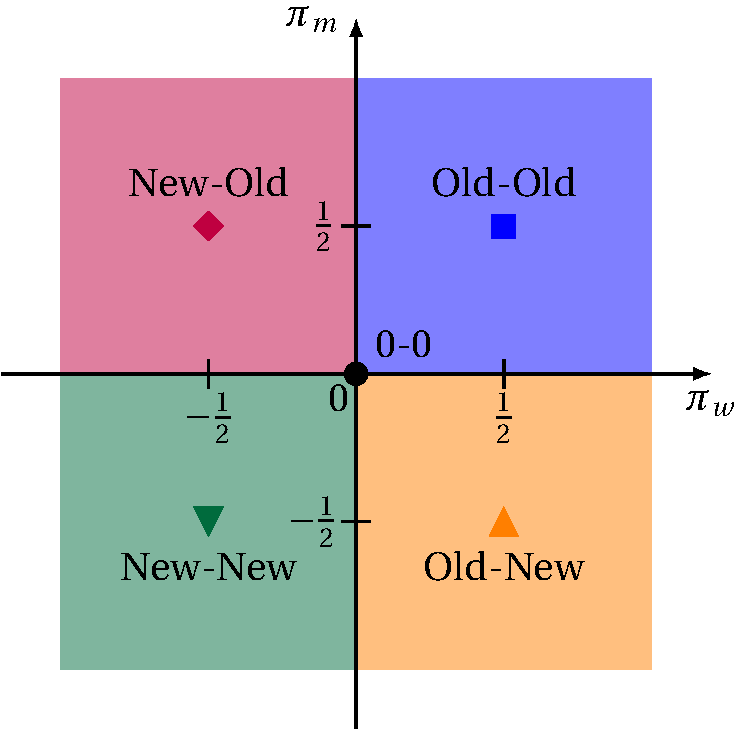
\includegraphics[width=0.5\textwidth]{fig1.pdf}
    \caption{\textbf{Parameter sets for the different dispersal schemes.} \small The colors and markers are the same across all figures. The $x$ and $y$ axes show the dispersal bias of the wild type and mutant, respectively, to immigrate into old-habitat patches ($\pi_w$ and $\pi_m$). The markers are located at the parameter values used for the simulations: $\pi_m=\pi_w=0$ for unbiased dispersal (0-0; {\Large $\bullet$}), $\pi_m=\pi_w=0.5$ for a type-independent bias towards old-habitat patches (Old-Old; {\color{blue} $\blacksquare$}), $\pi_m=-0.5,\pi_w=0.5$ for a wild-type preference towards the old habitat, and a mutant-bias to the new habitat (Old-New; {\color{orange}$\blacktriangle$}), $\pi_m=\pi_w=-0.5$ for a type-independent bias towards the new habitat (New-New; {\color{darkgreen}$\blacktriangledown$}), and $\pi_m=0.5,\pi_w=-0.5$ for the mutant-bias towards the old habitat and a preference of the wild type for the new habitat (New-Old; {\color{purple}$\blacklozenge$}). All the results derived below depend continuously on these parameters, so that varying any of the parameters will not result in a sudden change or discontinuity of the corresponding curves. {\color{orange} Do we need this last sentence?\color{blue}No.}}
    \label{fig:disp_schemes}
\end{figure}

\linespread{1}
\begin{table}[t!]
	\begin{center}
		\begin{tabular}{c | P{6cm} | c | c}
			\textbf{Parameter} & \textbf{Interpretation} & \textbf{Range} & \textbf{Default value} \\
			\midrule
			$K_k$ & Carrying capacity in a patch of type $k$ & -- & \makecell{$K_{\text{old}}=1000$,\\ $K_{\text{new}}=500$} \\
			$\omega_j$ & \makecell{Expected per-capita number of\\ type $j$ offspring in the old habitat\\ before regulation} & $0\leq \omega_m < \omega_w$ & \makecell{$\omega_w = 1.5$,\\ $\omega_m=1.45$ {\footnotesize (weak sel.)},\\ $\omega_m=1.35$ {\footnotesize (strong sel.)}}\\
			$1+a_{\text{old}}$ & \makecell{Growth rate of the mutant\\ in the old habitat} & $-1\leq a_{\text{old}}$ & -- \\
			$1-r$ & \makecell{Mean number of wild-type offspring\\ in the new habitat} & $0<r\leq 1$ & \makecell{$0.75$\\ $(r=0.25)$}\\
			$1+a_{\text{new}}$ & \makecell{Growth rate of the mutant\\ in the new habitat} & $0<a_{\text{new}}$ & \makecell{$1.02$ \\ ($a_{\text{new}}=0.02$)} \\
			$m$ & Emigration probability & $0<m\leq 1$ & $0.06$\\
			$\pi_i$ & Type $i$ bias towards the old habitat & $\pi_i\in\mathbb{R}$ & see Fig.\ref{fig:disp_schemes}\\
			$\widehat{\pi}_i$ & Transformed dispersal bias of type $i$ & $0<\widehat{\pi}_i$ & see Fig.\ref{fig:disp_schemes}\\
			$M$ & Number of patches & $2\leq M$ & $10$\\
			$f_{\text{old}}$ & Frequency of old-habitat patches & $0\leq f_{\text{old}}\leq 1$ & $0.5$ \\
			$\theta$ & Mutation probability & $0 < \theta$ & $\frac{1}{25 M K_{\text{new}}}$\\
			$\tau$ & Time interval between two consecutive deterioration events& $0<\tau$ & $100$\\
			\midrule
			$\widehat{N}_{i}^{k}$ & \multicolumn{3}{p{11cm}}{Number of type $i$ individuals in type $k$ habitat patches at stationarity}  \\
			$\widetilde{N}_{i}^{k}$ & \multicolumn{3}{p{11cm}}{Number of type $i$ individuals in type $k$ habitat patches after dispersal}
		\end{tabular}
		\caption{\textbf{Model parameters.}}	
		\label{tab:parameters}
	\end{center}
\end{table}
\linespread{1.7}

All the model parameters are summarized in Table~\ref{tab:parameters} along with the default parameter values and ranges. If not stated otherwise, the default parameter values are used for the stochastic simulations. 

\subsection*{Simulations}
The algorithm implements the life cycle described above. First, a random number of dispersing individuals \chg{from each patch} is drawn from a binomial distribution with success probability $m$ and sample size equal to the \chg{current patch} population size. The dispersing individuals \chg{are pooled and} distributed according to their type and the dispersal pattern. \linelabel{R2-18}\chg{More precisely, we draw a binomial number of individuals of each type to immigrate into an old-habitat patch with probability $\frac{m_i^{\text{old}}}{m}$ (eq.~\eqref{eq:dispersal}) and then distribute these individuals uniformly at random over the old-habitat patches. The same is done with the remaining dispersing individuals who are distributed uniformly into the new-habitat patches.} \linelabel{R2-19}\chg{In each patch, reproduction is simulated by drawing a Poisson distributed number for each type. The mean of this Poisson number is given by the number of individuals of type $i$ in that patch times the mean number of offspring of a single individual of type $i$ which depends on the patch type (old or new).} 
Mutation of the wild-type \linelabel{R2-20}\chg{offspring} \chg{happens} with \chg{probability} $\theta$, implemented using a binomial distribution. Lastly, if necessary, \linelabel{R1-25}\chg{patches are down-regulated back to carrying capacity by sampling individuals uniformly at random without replacement from the population in a patch until the carrying capacity is reached (hypergeometric sampling).} 

In Figs.~\ref{fig:vary_m_est}-\ref{fig:origin}, we simulate a heterogeneous environment that is constant in time, i.e. no patches deteriorate. Initial population sizes are $K_{\text{old}}$ wild-type individuals in old-habitat patches, and the \footnote{\francois{add `analytical' or `theoretical'}}stationary wild-type population size $\widehat{N}_w^{\text{new}}$ in new-habitat patches (see Section S1 in the SI for details). \chg{Simulations for} Fig.~\ref{fig:vary_m_est} are started with initially one mutant either in a old- or a new-habitat patch and the corresponding wild-type population size is reduced by one, \chg{and} the mutation probability is set to zero. In \linelabel{R2-21}\chg{Figs.~\ref{fig:source_sink} and \ref{fig:origin}}, mutants solely arise due to mutations \chg{over a finite time period}. 
We \chg{call the mutant established if} the total number of mutants in all new-habitat patches exceeds $0.\chg{6} \times K_{\text{new}} \times M(1- f_{\text{old}})$\footnote{\francois{These thresholds are mysterious at this stage.}} (\chg{or in old-habitat patches $0.6\times K_{\text{old}}\times M f_{\text{old}}$ which is relevant for dispersal schemes where the mutant has a bias towards old-habitat patches, Old-Old and New-Old}).
In the rescue scenario, where one patch after \chg{another} deteriorates (Figs.~\ref{fig:rescue} and \ref{fig:sgv}), we initialize all patches with $K_{\text{old}}$ wild-type individuals. Simulations are run until either the population has gone extinct or the (global) mutant population size exceeds $0.6\times K_{\text{new}}\times M$ after the last deterioration event has happened. 

Unless stated otherwise, the simulation results are averages of $10^5$ independent runs. All simulations are written in the C++ programming language and use the \textit{Gnu Scientific Library}. The codes and data to generate the figures are deposited on Gitlab\footnote{https://gitlab.com/pczuppon/evolutionary\_rescue\_and\_dispersal}.

%%%%%%%%%%%%%%%%%%%%%%%%%%%%%%%%%%%%%%%%%%%%%%%%%%%%%%%%%%%%%%%%%%%
%%%%%%%%%%%%%%%%% RESULTS %%%%%%%%%%%%%%%%%%%%%%%%%%%%%%%%%%%%%%%%%
%%%%%%%%%%%%%%%%%%%%%%%%%%%%%%%%%%%%%%%%%%%%%%%%%%%%%%%%%%%%%%%%%%%
\section*{Results}

We investigate the effect of the different dispersal schemes on the probability of successful adaptation and evolutionary rescue. We first compute the \textit{establishment probability} of a single mutant individual arising either in an old- or in a new-habitat patch. We then link this probability to the dynamics of a source-sink system, i.e. a fixed environment with a certain number of old habitats (sources) and new-habitat patches (sinks). We derive an expression for the probability of a mutation to emerge and establish in a given time interval. We call this second quantity the \textit{probability of adaptation}. Lastly, we study the time-varying scenario where patches, one after \chg{another}, deteriorate. We consider a third quantity, the \textit{probability of evolutionary rescue}, which corresponds to the probability that a mutant appears by mutation and establishes in the new environment \chg{after} all patches have deteriorated. The theoretical results are complemented by stochastic simulations that support our predictions and help visualize the differences between the different dispersal schemes.

%%%%%%%%%%%%%%%%%%%%%%%%%%%%%%%
% Establishment Probability %%%
%%%%%%%%%%%%%%%%%%%%%%%%%%%%%%%
\subsection*{Establishment probability in a heterogeneous environment}\label{subsec:establishment}

We derive the probability of establishment of a mutant population starting with a single individual initially located either in an old- or a new-habitat patch. In this analysis, we ignore further mutations and are only concerned with the fate of this single mutant lineage. 
The dynamics of the mutant population can be described by a two-type branching process, i.e. \linelabel{R1-27}\chg{all mutants, the descendants of the initial mutant, reproduce, disperse and die independently of each other.} This is a reasonable assumption as long as the overall number of mutants is a lot smaller than the population size of the wild type. The two ``types'' of the two-type branching process correspond to the two habitat types. The process tracks the \linelabel{R2-25}\chg{total number of mutants in old- and new-habitat patches at the end of the life cycle.} The number of offspring of a single mutant can be approximated by Poisson distributed numbers (see eq.~\eqref{eq:sold}). The mean number of offspring of a single mutant, either in an old- or a new-habitat patch, is then given by the following mean reproduction matrix:
%
\begin{equation}\label{eq:mean_repro}
	\bordermatrix{ ~ & \text{old patch} & \text{new patch} \cr
		\text{old patch} & \left(1-m_m^{\text{new}}\right) (1+a_{\text{old}}) & m_m^{\text{new}} (1+a_{\text{new}}) \cr
		\text{new patch} & m_m^{\text{old}} (1+a_{\text{old}}) & \left(1-m_m^{\text{old}}\right) (1+a_{\text{new}})
		}\ ,
\end{equation}
%
where the rows denote the parent locations, and the columns the patch type of the offspring. 
For example, the top-left entry reads as the probability for the parent to stay in an old-habitat patch ($1-m_m^{\text{new}}$) times the average number of offspring in these patches, given by the mean of the corresponding Poisson distribution with rate $(1+a_{\text{old}})$, cf. eq.~\eqref{eq:sold} \linelabel{R2-26}\chg{(see Section S1 in SI for the derivation of $a_{\text{old}}$ at the wild-type equilibrium)}. The other entries are obtained analogously.

\linelabel{R1-24}The survival probability of this multi-type branching process, $\varphi_{k}$ with $k$ indicating the initial habitat type of the mutant, is then given by the unique positive solution of the following system of equations \citep[see][Chapters 5.3 and 5.6]{haccou_book}
\begin{equation}\label{eq:ext_prob}
	\begin{aligned}
		1-\varphi_{\text{old}} &= \sum_{j=0}^{\infty}\left( \mathbf{P}(j \text{ offspring in old habitat})(1-\varphi_{\text{old}})^j \right. \\
		&\qquad \qquad \qquad \left.+ \mathbf{P}(j \text{ offspring in new habitat})(1-\varphi_{\text{new}})^j\right)\\
		&=\exp\left[-\left(1-m^{\text{old}\to \text{new}}_m\right)(1+a_{\text{old}})\varphi_{\text{old}} - m^{\text{old}\to \text{new}}_m (1+a_{\text{new}}) \varphi_{\text{new}}\right]\, ,   \\
		1-\varphi_{\text{new}} &= \exp\left[-m^{\text{new}\to \text{old}}_m(1+a_{\text{old}})\varphi_{\text{old}} - \left(1-m^{\text{new}\to \text{old}}_m\right) (1+a_{\text{new}}) \varphi_{\text{new}}\right]\, .
	\end{aligned}
\end{equation}
Intuitively the left hand side, the extinction probability, equals the sum over all possible scenarios of the trajectories towards extinction, e.g. the initial individual having $j$ offspring in a patch of type $k$, old or new, and all of these $j$ offspring becoming extinct ($(1-\varphi_{\text{k}})^j$). Unfortunately, a general analytical solution to these equations is not accessible, but they can be solved numerically. For weak selection and (potentially) weak dispersal -- i.e. $a_{\text{old}},a_{\text{new}},m\ll 1$ needs to hold for at least two of the three parameters -- an approximation is available: see for example~\citet[Theorem~5.6]{haccou_book} for the general theory and \citet{tomasini_2018} for an application in a similar setting. The detailed derivation is presented in the SI, Section~S2. We find
\begin{equation}\label{eq:estab_approx}
	\begin{aligned}
		\varphi_{\text{old}} &\approx \qquad \quad \; \; \; \; a_{\text{old}}&+ & \quad a_{\text{old}} \frac{\left(1-f_{\text{old}}+\widehat{\pi}_m f_{\text{old}}\right)}{\sqrt{C}}(a_{\text{old}}-a_{\text{new}}) \\
		& & &  \; \; \; + \; \frac{m}{\sqrt{C}} \left(a_{\text{new}}(1-f_{\text{old}}) + a_{\text{old}}\widehat{\pi}_m f_{\text{old}} - (a_{\text{old}}-a_{\text{new}})(1-f_{\text{old}})\right) \, ,\\
		\varphi_{\text{new}} &\approx \underbrace{ a_{\text{new}}}_{\text{(1) local growth parameter}} &+ & \quad \underbrace{ a_{\text{new}} \frac{\left(1-f_{\text{old}}+\widehat{\pi}_m f_{\text{old}}\right)}{\sqrt{C}}(a_{\text{new}}-a_{\text{old}})}_{\text{(2) effect of the heterogeneous environment}} \\
	& & &  \underbrace{+\; \frac{m}{\sqrt{C}}\left( a_{\text{new}}(1-f_{\text{old}}) + a_{\text{old}} \widehat{\pi}_m f_{\text{old}} - (a_{\text{new}}-a_{\text{old}}) \widehat{\pi}_m f_{\text{old}} \right)\, ,}_{\text{(3) effect of dispersal: new patches $+$ old patches $-$ loss to the other patch type }}
	\end{aligned}
\end{equation}
where $C$ is a scaling constant that depends on $m,f_{\text{old}},\widehat{\pi}_m,a_{\text{old}}$ and $a_{\text{new}}$ through
\begin{equation}\label{eq:normalization}
	C = (1-f_{\text{old}}+\widehat{\pi}_m f_{\text{old}}) \left((1-f_{\text{old}})(a_{\text{new}}-a_{\text{old}}+m)^2 + \widehat{\pi}_m f_{\text{old}} (a_{\text{new}}-a_{\text{old}}-m)^2\right)\, . 
\end{equation}

The first term in the approximation of the establishment probabilities ($\varphi_{\text{old}}$ and $\varphi_{\text{new}}$) in eq.~\eqref{eq:estab_approx} describes the local growth depending on the habitat type under study. 
The second term captures the growth rate differences between the two habitat types.
The factor $(1-f_{\text{old}}+\widehat{\pi}_m f_{\text{old}})$ accounts for the biased dispersal patterns (when $\pi_m\neq 0$ so that $\widehat{\pi}_m\neq 1$). 
The third term in the equations corresponds to the direct effect of dispersal on the establishment probability. 
The first two summands in the bracket are the same for both establishment probabilities. They represent the general effect of dispersal due to the dynamics from new-habitat patches (first summand) and old-habitat patches (second summand). The dispersal bias induced by $\pi_m$ changes the relative impact of old- vs. new-habitat patches. 
Finally, the last summand in the bracket measures the growth rate loss (or gain) due to dispersal to the other patch type. It therefore differs between the two approximations.

Note that in these equations, the competition of the mutant with the wild type in old-habitat patches appears in the local growth rate $a_{\text{old}}$, defined in eq.~\eqref{eq:sold}. This quantity is not constant, but instead depends on the wild type population size in old-habitat patches, which itself depends on the wild type's dispersal and growth rate in both habitats \linelabel{R2-28}\chg{(see SI, Section S1)}.

If the emigration probability is zero ($m=0$), the subpopulations in each habitat evolve in isolation from each other and we recover Haldane's classical result for the establishment probability of a slightly advantageous mutant in new habitats: $\varphi_{\text{new}}=2a_{\text{new}}$ \citep{haldane_1927}. \linelabel{R1-69}\chg{In old-habitat patches, where the mutation is deleterious, we see that term (1) and (2) cancel each other so that the establishment probability is simply $\varphi_{\text{old}}=0$.} Furthermore,\francois{when the emigration probability is strictly positive (m>0)} in the case of \chg{unbiased} dispersal ($\pi_w=\pi_m=0$) and for equal number of old- and new-habitat patches ($f_{\text{old}}=1/2$), we obtain the approximation found in \cite{tomasini_2018} (compare system~\eqref{eq:estab_approx} to their eqs.~(4) and~(5)). Note that the approximation is independent of the actual number of patches, but only depends on the environmental configuration determined by the frequency of old-habitat patches $f_{\text{old}}$.

\subsubsection*{Comparison to simulations and qualitative behavior}
We compare in Fig.~\ref{fig:vary_m_est} our predictions from eqs.~\eqref{eq:ext_prob} and~\eqref{eq:estab_approx} to simulation results for different values of the emigration rate $m$. We find good agreement with the numerical solution of eq.~\eqref{eq:ext_prob} (solid lines). The approximation given in eq.~\eqref{eq:estab_approx} (dashed lines) deviates slightly from the simulation results in regions where $m,a_{\text{new}}$ and $a_{\text{old}}$ are not small, i.e. when the assumptions made in the analytical derivation do not hold anymore. 

\begin{figure}[t!]
	\centering
	\begin{subfigure}{.5\textwidth}
  		\centering
  		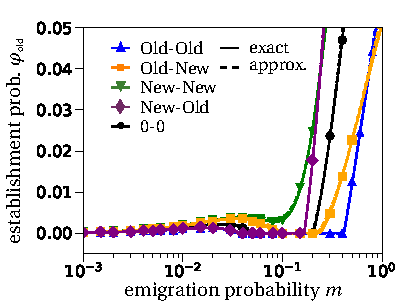
\includegraphics[width=\linewidth]{fig2a.pdf}
  		\caption{$\varphi_{\text{old}}$ with $\omega_m = 1.35$ (large fecundity difference)}
	\end{subfigure}%
	\begin{subfigure}{.5\textwidth}
 		 \centering
 		 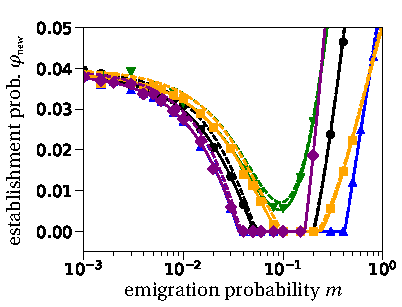
\includegraphics[width=\linewidth]{fig2b.pdf}
  		\caption{$\varphi_{\text{new}}$ with $\omega_m = 1.35$}
	\end{subfigure}
	\begin{subfigure}{.5\textwidth}
  		\centering
  		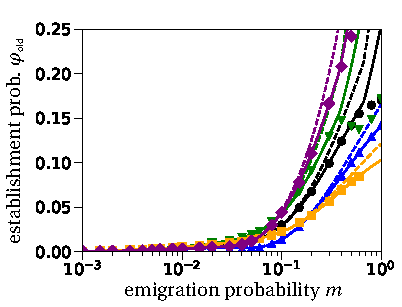
\includegraphics[width=\linewidth]{fig2c.pdf}
  		\caption{$\varphi_{\text{old}}$ with $\omega_m = 1.45$ (small fecundity difference)}
	\end{subfigure}%
	\begin{subfigure}{.5\textwidth}
 		 \centering
 		 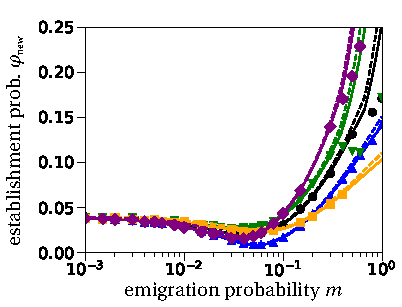
\includegraphics[width=\linewidth]{fig2d.pdf}
  		\caption{$\varphi_{\text{new}}$ with $\omega_m = 1.45$}
	\end{subfigure}
	\caption{\textbf{Establishment probability when varying the emigration rate.} \small We plot the theoretical results for $\varphi_{\text{old}}$ in (a) and (c), and for $\varphi_{\text{new}}$ in (b) and (d) for $\omega_m=1.35$ in (a), (b) and $\omega_m=1.45$ in (c), (d). Comparison with the results from stochastic simulations (symbols) show very good agreement with our approximation found in eq.~\eqref{eq:estab_approx} (dashed lines). The solid lines are the numerical solution of eq.~\eqref{eq:ext_prob}. The lines in (a) show a clear separation of the three regions of the establishment probability as discussed in the main text: {\color{change}(i) an initial increase due to higher probabilities of dispersal from old- to new-habitat patches; (ii) a local maximum due to increasing number of mutants emigrating from new-habitat patches; (iii) an increase due to relaxed competition in old-habitat patches, a result of wild-type emigration.}}
	\label{fig:vary_m_est}
\end{figure}

The qualitative dependence of the establishment probabilities $\varphi_{\text{old}}$ and $\varphi_{\text{new}}$ on the dispersal probability $m$ is similar for all dispersal schemes. The shape of the curve however strongly depends on the fecundity $\omega_m$ of mutants in the old habitat. Before discussing the differences between the dispersal schemes, we first provide a qualitative understanding of this general behavior.

For the probability of establishment of a single mutant in an old-habitat patch ($\varphi_{\text{old}}$), we observe up to three different regions, cf. Fig.~\ref{fig:vary_m_est}(a). This is in line with previous observations in the context of local adaptation \citep[e.g.][]{kawecki_1995,tomasini_2018} and evolutionary rescue \citep{uecker_2014}. We define the regions as follows: (i) an initial increase of the establishment probability at low dispersal rates $m$; (ii) a local maximum with a subsequent decrease of the establishment probability; (iii) an increase of the establishment probability for high dispersal rates.

A detailed assessment and explanation of the regions is provided in the SI, Section S2.1. Briefly, in region (i), the prevalent effect is the dispersal of mutants from old- to new-habitat patches where they are fitter than the wild type, thus increasing the establishment probability. This effect is mediated through the third term of the establishment probability in eq.~\eqref{eq:estab_approx}. 
Region (ii), beginning with the local maximum, is a result of two counteracting processes: %increased emigration of individuals from the old habitat and \linelabel{R2-30-1}\chg{an increasing probability of an individual that is born in a new habitat emigrates to an old-habitat patch.}
\linelabel{R2-30-1}\chg{If we increase the emigration probability $m$, a mutant is more likely to emigrate out of old-habitat patches and thus has a higher chance to establish. However, higher dispersal rates also have a negative effect on mutant establishment through \linelabel{R2-32}increasing the probability that a mutant migrates from a new- to an old-habitat patch. More precisely, the number of offspring in the new habitat on average is given by the product of the terms $(1-m_m^{\text{old}})$ and $(1+a_{\text{new}})$. This product can, for large emigration probabilities $m$, be smaller than $1$, i.e. a mutant in a new-habitat patch has on average less than one offspring. Finally, in region (iii), dispersal is so large that the population is close to being well-mixed. Most importantly, many wild-type individuals leave old-habitat patches which results in less competitive pressure in old-habitat patches. In this case the local growth rate of the mutant in these patches, $a_{\text{old}}$ (first term in eq.~\eqref{eq:estab_approx}), becomes positive. This effect called `relaxed competition'~\citep{uecker_2014}. The onset of this effect, in terms of the emigration probability $m$, is strongly dependent on the fecundity values of the mutant in the old habitat. The larger it is, the `earlier' (i.e. for smaller emigration rates $m$) relaxed competition becomes relevant.} 

%lowering competitive pressure in old-habitat patches \linelabel{R1-28-1}(see $\widetilde{N}_{\text{old}}^w$ from eqs.~(S7) and~(S8) in the SI). As a result, local growth rates of the mutant in old-habitat patches, \linelabel{R1-30} $a_{\text{old}}$, become larger. This effect was termed `relaxed competition' by \citet{uecker_2014}. 

%Depending on the onset of this effect, the establishment probability either has a local maximum or not, compare \ref{fig:vary_m_est}(a) and (c).
 
\chg{In line with this reasoning we find} that the width of region (ii) strongly depends on the fecundity of the mutant in the old habitat, $\omega_m$. If $\omega_m$ is high, the local growth rate of the mutant $a_{\text{old}}$ starts to increase at a lower dispersal rate 
%(see Fig.~S1). 
\chg{and }region (ii) disappears, as visible in Fig.~\ref{fig:vary_m_est}(c). In contrast, for low mutant fecundity values $\omega_m$, region (iii) might vanish (see Fig. S2 in SI). There, the mutant is strongly disadvantageous in old-habitat patches when compared to the wild type, and the wild-type population will always outcompete the mutant due to the much higher offspring numbers.

We analyze the qualitative behavior of the establishment probability of a mutant emerging in the new habitat, $\varphi_{\text{new}}$ in a similar way (Figs.~\ref{fig:vary_m_est}(b,d)). The establishment probability $\varphi_{\text{new}}$ decreases at low dispersal rates: Since we let the mutant start in a new-habitat patch, where it fares better than the wild type, there is no initial benefit due to dispersal (the third term in eq.~\eqref{eq:estab_approx} is negative for $\varphi_{\text{new}}$). The interpretation of region (ii), describing the trajectory for intermediate emigration rates $m$, is the same as for $\varphi_{\text{old}}$ above. For large emigration rates $m$, region (iii), the resulting establishment probability is a combination of the local growth rate and the dispersal effect, the first and third terms in eq.~\eqref{eq:estab_approx}. This is because the mutant can migrate to old-habitat patches, where it will enjoy relaxed competition. %%

\chg{Lastly, for large emigration probabilities $m$ in Fig.~\ref{fig:vary_m_est}(c,d) we observe a decrease in the establishment probability of the simulation results of the New-New dispersal scheme (and to a lesser extent in the unbiased scheme). This is explained by `gene swamping' whereby a to large number of immigrants of a less-well adapted type (wild type) inhibits the establishment of a locally better adapted type (mutant) \citep{nagylaki_1978,lenormand_2002}. Here, gene swamping occurs because of the different carrying capacities of the two patch types, $K_{\text{new}}<K_{\text{old}}$. A proper analysis of the gene swamping regime, where density-dependence in new-habitat patches is important, is beyond the scope of this manuscript, but see for instance \citet{tomasini_2018} and Section S5 in the SI where such a situation is studied.}\footnote{\pete{If I do not mention gene swamping here, I think people will wonder what this effect is and misinterpret it as a late relaxed competition effect.}}

\subsubsection*{Comparison of dispersal schemes}

We now compare the establishment probabilities for the different dispersal schemes. 
We consistently observe that \chg{a bias towards the new habitat (New-New} in Fig.~\ref{fig:vary_m_est}) enhances establishment when compared to the \chg{unbiased} dispersal scheme (0-0). This can be attributed to two reasons: (1) the mutant is more likely to disperse to the new habitat where it outcompetes the wild type (stronger weighting of new-habitat patches in the third term in eq.~\eqref{eq:estab_approx}); and (2) since the wild type prefers to settle in new-habitat patches ($\pi_w<0$), individuals in old-habitat patches experience relaxed competition for lower dispersal rates $m$, thus increasing the local growth rate $a_{\text{old}}$, i.e. region (iii) is shifted to the left. An analogous (but reversed) argument explains why \chg{a bias towards the old habitat (Old-Old}) is always lower than the \chg{unbiased} dispersal scheme. 

The effect of \chg{the asymmetric dispersal scheme Old-New}, where each type has a bias to move to the habitat where it is relatively fitter than the other type, is more involved. We disentangle the effects separately for each region. In region (i) at low emigration probabilities, the curve is almost identical to that of the \chg{New-New} pattern. The mutant preference \chg{(new habitats)} of these two dispersal modes is the same. The movement of the rare mutant is the prevailing process in this parameter regime, which explains the alignment of the \chg{corresponding} curves. 
For intermediate dispersal rates, region (ii), the effect of the heterogeneous environment (second term in eq.~\eqref{eq:estab_approx}) becomes stronger, i.e. the local growth rate $a_{\text{old}}$ increases because of relaxed competition in old-habitat patches. 
For the \chg{Old-New scheme}, the\linelabel{R2-30-3} wild type is more likely to immigrate into old-habitat patches and to increase the population size in these locations \linelabel{R1-31}\chg{when compared to the New-New dispersal scheme}. This reduces the effect of relaxed competition. Therefore, the \chg{Old-New line} drops below the \chg{New-New} curve and even starts to decrease (Fig.~\ref{fig:vary_m_est}(a)). For high emigration probabilities $m$, region (iii), the competitive pressure in old-habitat patches relaxes. Again, this region is dominated by the movement of wild-type individuals. In the \chg{unbiased} dispersal scheme, the wild type has a lower likelihood to be in old-habitat patches than with the \chg{Old-New} scheme, explaining the \chg{order of these} curves. 
For very large dispersal rates, also\francois{moreover?} the \chg{Old-Old} scheme can lead to higher values of $\varphi_{\text{old}}$ than \chg{the type-dependent preference Old-New}, cf. Fig.~\ref{fig:vary_m_est}(c). For these parameters, the mutant has a larger growth rate in old- than in the new-habitat patches ($a_{\text{old}}>a_{\text{new}}$). It is therefore beneficial for the mutant to \linelabel{R2-30-4}\chg{be in} old-habitat patches. 

Finally, for the \chg{asymmetric dispersal scheme New-Old, where the types have a bias to the habitat they are less well adapted to, }we see that for low dispersal rates $m$ the results match those obtained under the \chg{Old-Old} scheme. The mutant preferences being the same, this again shows that this region is dominated by the mutant's dispersal behavior. For intermediate to large dispersal rates though, the \chg{New-Old} scheme results in the largest establishment probabilities. This is explained by the effect of strongly relaxed competition (wild-type individuals preferentially move into the new habitat) and the bias of mutants to disperse into old-habitat patches where their number of offspring individuals is now very large. %Overall, this results in the highest establishment probabilities of all dispersal schemes. %We note though that the term `maladaptive dispersal' might be misleading for large dispersal values, since here the growth rate of the mutant in old-habitat patches, $a_{\text{old}}$, is actually larger than the growth rate in new-habitat patches, $a_{\text{new}}$. 

%%%%%%%%%%%%%%%%%%%%%%%%%%%%%%%
% Emergence probability %%%%%%%
%%%%%%%%%%%%%%%%%%%%%%%%%%%%%%%
\subsection*{Probability of adaptation in a heterogeneous environment} \label{subsec:source_sink}

We now study the probability of adaptation when mutations occur recurrently. As in the previous section, we consider a heterogeneous environment with a fixed number of old- and new-habitat patches. This is effectively a source-sink system \citep{holt_1985,pulliam_1988}, where old- and new-habitat patches correspond to sources and sinks for the wild type, respectively. In the previous section, we initialized the system with one mutant in either an old- or a new-habitat patch and computed the establishment probability. Now, we let mutants appear randomly within a certain time frame. The last time point at which a mutation can occur is denoted by $t_{\text{fin}}$.
Later, in the analysis of the probability for evolutionary rescue, this time will be replaced by the time between two consecutive patch deterioration events, $\tau$.\footnote{\pete{I think we can get rid of this last sentence. Thoughts?}\francois{Yes.}}

The probability of adaptation in this setting, $P_{\mathrm{adapt}}$, is given by
\begin{equation}\label{eq:source_sink}
	P_{\mathrm{adapt}} = 1 - \exp\left(-\theta t_{\text{fin}} M \left(\underbrace{\varphi_{\text{old}} f_{\text{old}} K_{\text{old}}}_{\text{old habitat contribution}} + \underbrace{\varphi_{\text{new}} (1-f_{\text{old}}) \widehat{N}_w^{\text{new}}}_{\text{new habitat contribution}}\right)\right)\, .	
\end{equation}
In words, the right-hand side is one minus the probability of no mutant establishing within the $[0, t_{\text{fin}}]$ time interval.
More precisely, the exponential is the probability of zero successes of a Poisson distribution. The rate of this Poisson distribution is given by the expected number of successfully emerging mutant lineages until time $t_{\text{fin}}$. \linelabel{R2-34}\chg{Assuming a Poisson distribution for the number of successful mutant lineages is an approximation of a Binomial distribution with large sample size (the wild-type populations $t_{\text{fin}} M f_{\text{old}} K_{\text{old}}$ in the old and approximately $t_{\text{fin}} M (1-f_{\text{old}}) \widehat{N}_w^{\text{new}}$ in the new habitats, see SI eq.~(S5)) with small success probability (the establishment probabilities $\varphi_{k}$). The sample size denotes the number of mutations in the system until time $t_{\text{fin}}$ and each of these mutants has, independently of each other (another approximation), has a survival probability of $\varphi_{k}$, dependent on the habitat it is born in.}
%Correctly, at least in the old habitat, one would have a Binomial distribution with success probability $\theta \varphi_{\text{old}}$ and sample size $t_{\text{fin}}M f_{\text{old}} K_{\text{old}}$ which is well approximated by a Poisson distribution for large sample sizes and small success probabilities. Due to the varying population size in the new habitat, the exact probability for successful lineages emerging from that habitat type is more difficult to compute. Yet again, on average this number is well approximated by the a Poisson distribution with a rate as stated above.}\footnote{\pete{This is the long explanation. I would shorten but if you think it is worth keeping a long explanation (as suggested by the reviewer) we can leave it as it is.}}
Note also, that for $t_{\text{fin}}$ tending to infinity, there will almost surely be a successful mutant so that $P_{\text{adapt}}=1$. \\
%For finite values of $t_{\text{fin}}$, the average number of mutations that appear until that time is given by the product of the mutation probability $\theta$, the length of the time window of interest $t_{\text{fin}}$, the number of patches $M$ and the stationary number of wild-type individuals present in the different habitats, that is $K$ and $\widehat{N}_w^{\text{new}}$ for old- and new-habitat patches, respectively (cf. SI eq.~(S5)). Once such a mutant appears, it then has the previously computed establishment probability $\varphi_{k}$ to establish, depending on the patch type $k$ (old or new) it arises in. This explains the factor $\varphi_k$ in the exponential.  \\

In Fig.~\ref{fig:source_sink} we compare our predictions to simulation results. The shape of the probability of adaptation as function of the emigration probability $m$ depends on the fecundity of the mutant in old-habitat patches, $\omega_m$ (Figs.~\ref{fig:source_sink}(a,c)). This is similar to the behavior of the establishment probability $\varphi_{\text{old}}$ in Fig.~\ref{fig:vary_m_est}. Likewise, the qualitative effects of the different dispersal schemes are comparable to the ones observed for the establishment probability. \linelabel{R1-33}\chg{This holds because the probability of adaptation, $P_{\text{adapt}}$, is given by $1-\exp(-C_1 \varphi_{\text{old}} -C_2 \varphi_{\text{new}})$ where two constants $C_1$ and $C_2$ depend on the dispersal scheme (see eq.~\eqref{eq:source_sink}). \linelabel{R2-35}The small differences in the ranking of the dispersal schemes between subfigures Figs.~\ref{fig:vary_m_est}(c) and Figs.~\ref{fig:source_sink}(c) can be explained by the mutational input, i.e. larger stationary populations sizes of the wild type in new habitats, $\widehat{N}_w^{\text{new}}$ result in more mutations during the observed time frame. This population size is altered by the different dispersal schemes, most importantly it is largest for the wild type having a bias towards old habitats, i.e. the Old-Old and the Old-New dispersal schemes.} 

\begin{figure}[t!]
	\centering
		\begin{subfigure}{.5\textwidth}
 		 \centering
 		 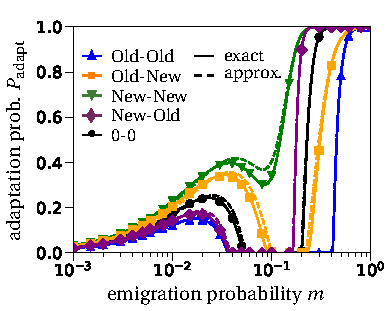
\includegraphics[width=\linewidth]{fig3a.pdf}
  		\caption{$\omega_m=1.35$ (large fecundity difference)}
	\end{subfigure}%
	    \begin{subfigure}{.5\textwidth}
 		 \centering
 		 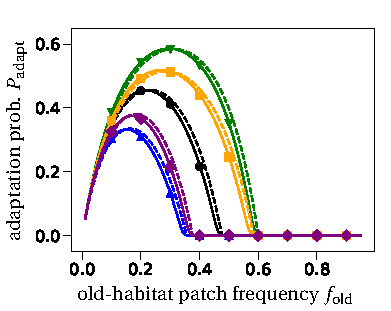
\includegraphics[width=\linewidth]{fig3b.pdf}
  		\caption{$\omega_m=1.35$}
	\end{subfigure}
	\begin{subfigure}{.5\textwidth}
 		 \centering
 		 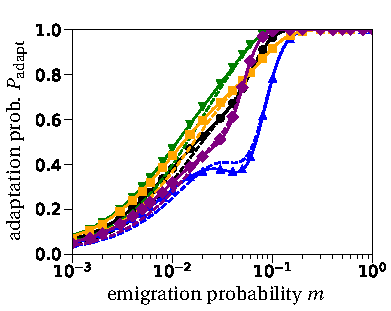
\includegraphics[width=\linewidth]{fig3c.pdf}
  		\caption{$\omega_m=1.45$  (small fecundity difference)}
	\end{subfigure}%
	\begin{subfigure}{.5\textwidth}
  		\centering
  		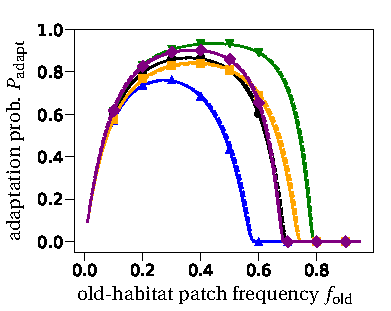
\includegraphics[width=\linewidth]{fig3d.pdf}
  		\caption{$\omega_m=1.45$}
	\end{subfigure}
	\caption{\textbf{Probability of adaptation in a heterogeneous environment.} \small In (a) and (c), we vary the emigration rate $m$ and observe a similar qualitative behavior as for the establishment probability $\varphi_k$ in Fig.~\ref{fig:vary_m_est}. In (b) and (d), we vary the frequency of old-habitat patches. The maximum is the result of two counteracting processes. The higher the number of old-habitat patches (the greater $f_{\text{old}}$), the larger the wild-type population. As a consequence, more mutants appear in the studied time-frame. In contrast, the less old-patch habitats there are in the environment (the lower $f_{\text{old}}$), the higher the probability of successful establishment of a mutant population. The curves labeled `approx.' are given by eq.~\eqref{eq:source_sink}, the exact solution refers to solving the establishment probabilities $\varphi_k$ from eq.~\eqref{eq:ext_prob} numerically and plugging these solutions into eq.~\eqref{eq:source_sink}. In all panels, the mutation probability is $u=1/(M K)$ and the final time for a mutant to appear is $t_{\text{fin}}=100$. }
	\label{fig:source_sink}
\end{figure}

In subfigures (b) and (d), we plot the probability of adaptation as a function of the frequency of old-habitat patches $f_{\text{old}}$. We observe a maximum which is the result of two effects: (1) the likelihood for a mutation to appear increases with the number of wild-type individuals present in the system, which is highest for high frequencies of old-habitat patches $f_{\text{old}}$, and (2) the probability of establishment of a mutant decreases with the number of old-habitat patches. 

The different dispersal schemes alter both effects. \chg{A general bias towards the new habitat (New-New)}, when compared to \chg{unbiased} dispersal (0-0), always shifts the maximum to higher frequencies of old habitats while also increasing its quantitative value. \chg{Since for the New-New dispersal scheme, both types prefer settling in new-habitat patches ($\pi_w,\pi_m<0$), the local population before reproduction in these patches is increased. Thus, the overall population size is higher compared to the other dispersal schemes and therefore a higher number of mutants is generated under this scheme.} Additionally, the probability of establishment is also increased for \chg{the New-New} dispersal scheme, further increasing the probability of adaptation (see also the discussion around Fig.~\ref{fig:vary_m_est}). Again, a reversed argument explains why \chg{the general preference for old-habitat patches (Old-Old)} always yields lower probabilities of adaptation than \chg{unbiased} dispersal.  


%%%%%%%%%%%%%%%%%%%%%%%%%%%%%%%
% Origin of rescue mutation %%%
%%%%%%%%%%%%%%%%%%%%%%%%%%%%%%%
\subsection*{Habitat of origin of the adaptive mutation}
We now identify the habitat type where the successful mutation arises. The established mutant population often arises from a single mutant that is born in an old- or in a new-habitat patch. However, the rescued population can sometimes be traced back to two (or more) mutant individuals, \chg{at least} one from either patch type. \linelabel{R1-35}\chg{This is a special type of a soft selective sweep \citep[see][for a review]{hermisson_2017}. The approximate probability to observe a soft sweep from mutants from both habitat types is 
\begin{equation}\label{eq:origin}
    \begin{aligned}
	&\mathbf{P}\big(\text{successful adaptation from old habitat}\big)\ \mathbf{P}\big(\text{successful adaptation from new habitat}\big) \\
	& \qquad \qquad \approx \left(1 - \exp\left(-\theta t_{\text{fin}} M \varphi_{\text{old}} f_{\text{old}} K\right)\right)\left(1- \exp\left(-\theta t_{\text{fin}} M \varphi_{\text{new}} (1-f_{\text{old}}) \widehat{N}_w^{\text{new}}\right)\right)\, .
	\end{aligned}
\end{equation} 
}
\linelabel{R1-36}\chg{The approximation uses our basic assumption that different mutant individuals and consequently also the offspring of different mutants do not affect each others dynamics (branching process). In the simulations, we label a run as a soft sweep from mutants arising in different locations if these lineages are still alive after $1000$ generations. This ensures that we do not count any false-positives where a mutant in one of the habitats has just arisen right before the mutant population exceeds the establishment threshold.}

%The probabilities for the other two scenarios can be computed analogously. 
In Fig.~\ref{fig:origin} we compare simulation results with our predictions for the origin of a successful mutant when varying the old habitat frequency $f_{\text{old}}$. \chg{\linelabel{R2-36}We see that for both mutant fecundity values most successful mutations arise in old-habitat patches. The difference in the input from the two different patches is the factor $\varphi_{k} \widehat{N}_w^k f_k$. In Fig.~SX we plot the establishment probability $\varphi_k$ and the stationary population sizes $\widehat{N}_w^k$ when varying the frequency of old-habitat patches $f_{\text{old}}$. We see that the establishment probability for mutants arising in new-habitat patches, $\varphi_{\text{new}}$, is always larger than the corresponding probability for mutants from old-habitat patches, $\varphi_{\text{old}}$. Conversely, the stationary population size of the wild type in the old habitat measured over the whole environment is always larger then that of the wild type in new habitats. Combining these two observations we find that for this choice of parameters the mutational input, i.e. the absolute number of rescue mutants, has a larger influence on the origin of the rescue mutant than the corresponding establishment probability.}

%Even for a relatively strong fecundity disadvantage of the mutant in the old habitat, i.e. $\omega_m$ is $10\%$ smaller than $\omega_w$, we find that most successful mutations arise in old-habitat patches (Fig.~\ref{fig:origin}(a)). Decreasing the fecundity disadvantage of the mutant by increasing its fecundity $\omega_m$ further increases the number of successful mutant lineages from old-habitat patches (Fig.~\ref{fig:origin}(b)). 
%If we instead increase the fecundity difference in old habitats by decreasing $\omega_m$, we observe the opposite, i.e. \chg{the two lines approach each other} (see Fig.~S4 in SI).

\begin{figure}[t!]
	\centering
	\begin{subfigure}{.5\textwidth}
 		 \centering
 		 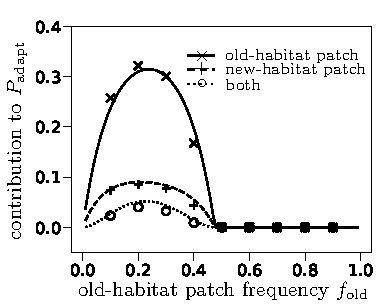
\includegraphics[width=\linewidth]{fig4a.pdf}
  		\caption{$w_m = 1.35$ (large fecundity difference)}
	\end{subfigure}%
	\begin{subfigure}{.5\textwidth}
  		\centering
  		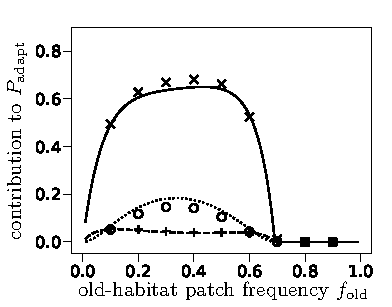
\includegraphics[width=\linewidth]{fig4b.pdf}
  		\caption{$w_m = 1.45$ (small fecundity difference)}
	\end{subfigure}
	\caption{\textbf{Origin of the adaptive mutant.} \small The origin of the adaptive mutant is strongly affected by the fecundity differences in the old habitat. If the difference is large as illustrated in panel (a), mutants appear more often in old-habitat patches than in new-habitat patches. Still, mutants arising in new-habitat patches contribute to the overall probability of adaptation. If fecundity differences are small like in panel (b), the successful mutant largely arises in old-habitat patches. In this case, the contribution from new-habitat patches is negligible. Circles correspond to simulations identified as soft selective sweeps with (at least) one lineage \francois{successful mutation} arising in an old- and one in a new-habitat patch. The curves are given by eq.~\eqref{eq:origin} (or the adjusted versions of it) under the unbiased dispersal scheme ($\pi_w=\pi_m=0$). Note the different scaling on the y-axes.}
	\label{fig:origin}
\end{figure}

%%%%%%%%%%%%%%%%%%%%%%%%%%%%%%%
% Evolutionary Rescue %%%%%%%%%
%%%%%%%%%%%%%%%%%%%%%%%%%%%%%%%
\subsection*{Evolutionary rescue}
Finally, we consider a time-inhomogeneous environment where patches deteriorate one after \chg{another} at regular time intervals $\tau$, until all patches have switched to the new habitat. If the wild-type population fails to generate a successful mutant, the population will \chg{inevitably} go extinct. The probability of evolutionary rescue is therefore tightly linked to the probabilities of adaptation and establishment that we have computed in eqs.~\eqref{eq:estab_approx} and~\eqref{eq:source_sink}. Typically, in formulas expressing the probability of evolutionary rescue, one splits the contributions into mutations arising \textit{de novo} and evolutionary rescue due to standing genetic variation, i.e. mutations that are present in the population before the environmental change \citep{alexander_2014}. We will discuss the effect of standing genetic variation in our system in the following section. For now, we focus on evolutionary rescue due to de novo mutations. We approximate the probability of evolutionary rescue, denoted by $P_{\text{rescue}}$, as
\begin{equation}\label{eq:evol_rescue}
    \begin{aligned}
		P_{\text{rescue}} &\approx 1-\exp\left(- \theta \sum_{i=0}^{M-2} \left(\underbrace{\varphi_{\text{old}}\left(f_{\text{old}}(i)\right) \sum_{j=i\tau}^{(i+1)\tau -1} N_w^{\text{old}}(j)}_{\text{old habitat contribution}} + \underbrace{\varphi_{\text{new}}(f_{\text{old}}(i)) \sum_{j=i\tau}^{(i+1)\tau -1} N_w^{\text{new}}(j)}_{\text{new habitat contribution}}\right)\right.\\
		&\qquad\qquad \qquad\qquad\qquad\qquad\qquad \qquad \qquad \qquad\quad  \left.\underbrace{-\theta \varphi_{\text{new}}(0) \sum_{j = \tau (M-1) }^\infty  N_w^{\text{new}}(j)}_{\text{contribution after the last patch deteriorated}}\right),
	\end{aligned}
\end{equation}
where \linelabel{R1-40}$f_{\text{old}}(i) = (M-i-1)/M$ is the frequency of old-habitat patches after the $(i+1)-$th deterioration event\linelabel{R1-39}\chg{, the establishment probability is given as a function of the patch frequency, $\varphi_k(f_{\text{old}}(i))$,} and $N_w^{k}(j)$ denotes the overall number of wild-type individuals living in habitat $k$ (old or new) in generation~$j$ \chg{(see SI, Section S1 for an approximation)}. The interpretation of this equation is the same as for eq.~\eqref{eq:source_sink}. The only difference is that we now need to account for a changing environment, which alters the population sizes, $N_w^k$, and the establishment probabilities $\varphi_k$ \chg{over time}. In the formula, these changes are accounted for by the sums that iterate through the (discrete) time steps and by the time dependence of the corresponding quantities. We further note that we follow the \chg{expected value of} the wild-type population size deterministically over time, instead of assuming it to be already in its steady state as in eq.~\eqref{eq:source_sink} \chg{(see also Section S1 in the SI)}.

As visible in Fig.~\ref{fig:rescue}, the approximation explains the \linelabel{R1-42}\chg{order of dispersal schemes}. Yet, it does not accurately predict the simulated data. This discrepancy can be explained: in the formula we \linelabel{R2-42}\chg{assume that for a mutant born in a certain patch configuration, say with $j$ old-habitat patches, the environment does not change anymore. That is, a mutant born in patch-type $k$ (old or new) in this environment contributes $\varphi_{k}(j)$ to the probability of evolutionary rescue despite further patches deteriorating. Thus, this mutants probability of establishment is underestimated. This is especially true for mutants that emerge just before a deterioration event. These mutants are more likely to establish during the subsequent environmental configuration giving them a higher probability of survival than approximated by our formula. Additionally, $\varphi_k(j)$ assumes stationary wild-type population sizes and therefore does not reflect the decreasing wild-type population size right after the deterioration of a patch.} 
%However, mutants that arise very shortly before a deterioration event just need to survive until this event happens and are thus carried over to the following environmental configuration with a higher probability than predicted by our formula. 
This explains why the simulation results are higher than our approximation. 
%which ignores these ``left-over'' mutants present prior to the deterioration event. 
\chg{A time-dependent establishment probability could account for these effects but unfortunately is not amenable to approximations in our framework.}
%As a result, instead of assuming a constant establishment probability between two deterioration events, we should rather use a time-dependent establishment probability -- which can however not be approximated in our general framework. 
\linelabel{R1-43}\chg{In \citet{uecker_2014}, scenarios with an accessible time-dependent solution were studied, more precisely situations with either full mixing of the global population ($m=1$) or a non-viable mutant in old-habitat patches ($\omega_m=0$).}

\begin{figure}[t!]
	\centering
	\begin{subfigure}{.5\textwidth}
  		\centering
  		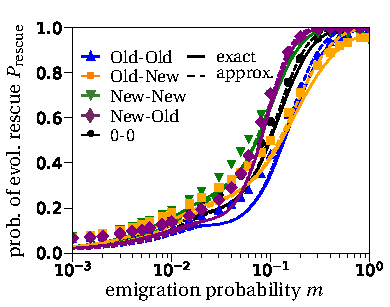
\includegraphics[width=\linewidth]{fig5a.pdf}
  		\caption{$\omega_m=1.45$ (small fecundity difference)}
	\end{subfigure}%
	\begin{subfigure}{.5\textwidth}
  		\centering
  		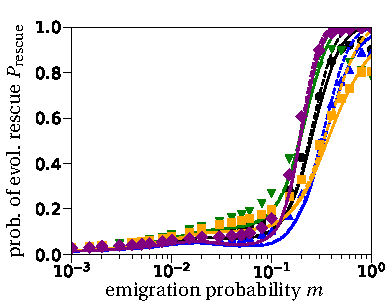
\includegraphics[width=\linewidth]{fig5b.pdf}
  		\caption{$\omega_m=1.35$ (large fecundity difference)}
	\end{subfigure}
	\begin{subfigure}{.5\textwidth}
  		\centering
  		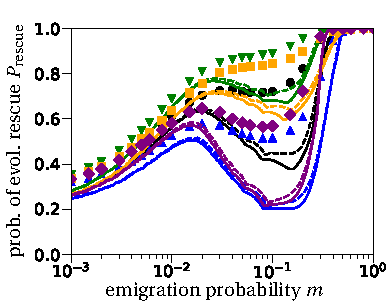
\includegraphics[width=\linewidth]{fig5c.pdf}
  		\caption{$\omega_m=1.1$ (very large fecundity difference)}
	\end{subfigure}%
	\begin{subfigure}{.5\textwidth}
  		\centering
  		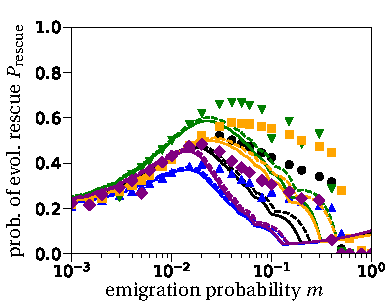
\includegraphics[width=\linewidth]{fig5d.pdf}
  		\caption{$\omega_m=0$ (lethal mutant)}
	\end{subfigure}
	\caption{\textbf{The probability of evolutionary rescue compared to simulation results.} \small Our predictions, computed with eq.~\eqref{eq:evol_rescue}, match the qualitative behavior of the simulated data for the probability of evolutionary rescue. All rankings of the dispersal schemes align well. Quantitatively though, we find that our predictions tend to underestimate the simulated data. In (a,b) the mutation probability is set to $u=1/(25MK_{\text{new}})$ while in (c,d) it is $u=1/(MK_{\text{new}})$. The label `exact' refers to the exact solution of eq.~\eqref{eq:ext_prob} which is then plugged into the approximation of the probability of evolutionary rescue in eq.~\eqref{eq:evol_rescue}.}
	\label{fig:rescue}
\end{figure}

The different dispersal schemes exhibit substantial differences. The dispersal schemes affect the dispersal pattern of both types and as such alter their respective population dynamics. Both small and large fecundity differences in the old habitat, $\omega_m=1.45$ and $\omega_m=1.35$, conserve the ranking of dispersal schemes obtained for the probabilities of establishment and adaptation\footnote{\francois{difficult to follow}\pete{We could also get rid of the explict description of the figure and remove the following sentence}}: \linelabel{R2-43}\chg{New-New (green) is higher than unbiased dispersal (black) which is higher than Old-Old (blue), with Old-New decreasing and New-Old increasing their positions with increasing emigration probability $m$}, cf. Fig.~\ref{fig:rescue}(a,b). Based on our discussion of the same behavior in Fig.~\ref{fig:vary_m_est}(a,c), \linelabel{R2-44}\chg{i.e. the change in hierarchy of the dispersal schemes Old-New and New-Old,} The most influential factor in these parameter sets is the growth rate of the mutant in old-habitat patches, $a_{\text{old}}$, \chg{as discussed around Fig.~\ref{fig:vary_m_est}.} \chg{The ranking of the symmetric dispersal schemes is mostly determined by the mutant dispersal bias.}

For very large fecundity differences in the old habitat ($\omega_m = 1.1$ and $\omega_m=0$), the ranking of dispersal schemes is the same for all emigration probabilities; from highest to lowest, we find \chg{New-New, Old-New, unbiased dispersal, New-Old, and Old-Old} (cf. Fig.~\ref{fig:rescue}(c,d)). In this parameter setting, the probability of evolutionary rescue is dominated by the dispersal behavior of the mutant. Since the mutant is barely viable in old-habitat patches, it is always preferential for it to disperse towards new-habitat patches. Two schemes follow this rule, \chg{the New-New and Old-New dispersal scheme}, but differ in the preference of the wild type. 
Since wild-type individuals also preferentially disperse to new-habitat patches under \chg{the New-New scheme}, more individuals are present in those patches. Therefore, the total amount of mutations over the deterioration time is increased which generates more mutants on average. This explains the New-New dispersal scheme being consistently higher than the Old-New dispersal scheme.
%This effect is even stronger for large dispersal rates that increase the wild-type population size in the whole environment. Together with the effect of relaxed competition, this explains the strong increase of the \chg{New-Old}, and the \chg{unbiased} dispersal scheme for large emigration probabilities $m$ in Fig.~\ref{fig:rescue}(c). 

Lastly, the probability of evolutionary rescue often reaches a local (or global) maximum for intermediate emigration probabilities (Figs.~\ref{fig:rescue}(c,d)). This extends previous results \citep{uecker_2014,tomasini_2019} to arbitrary dispersal schemes affecting the immigration process. The maximum can be attributed to the interaction of the three regions we identified when analyzing the establishment probability $\varphi_k$ (see also Fig.~\ref{fig:vary_m_est}). As such it is a result of the largely positive effect of dispersal (initial increase of the probability of evolutionary rescue) and the negative effect of population mixing \chg{(dispersal to old patches)}. \footnote{\francois{This discussion is still difficult.}}

\subsection*{Habitat of origin of the rescue mutant and standing genetic variation}
Similar to what \chg{we} found for the probability of adaptation, rescue mutants mainly originate from old-habitat patches. Mutations are more likely to appear in the more populated patches (old-habitat). However, a low mutant fecundity $\omega_m$ decreases the chance of establishment of these mutants that appear in old-habitat patches (compare black and yellow symbols in Fig.~\ref{fig:sgv}(a)). Lower fecundity values $\omega_m$ therefore comparatively increase the probability for the rescue mutation to have appeared in the already deteriorated habitat, i.e. in new-habitat patches. \linelabel{R1-35-2}\chg{The probability of a soft selective sweep for evolutionary rescue from mutants of the different habitat types is very low (circles in Fig.~\ref{fig:sgv}(a)). Our choice of a small mutation rate implies a hard selective sweep regime ($\theta K_{\text{old}} M = 0.08<1$) \citep{wilson_2018,hermisson_2017}. }

\begin{figure}[t]
	\centering
		\begin{subfigure}{.5\textwidth}
 		 \centering
 		 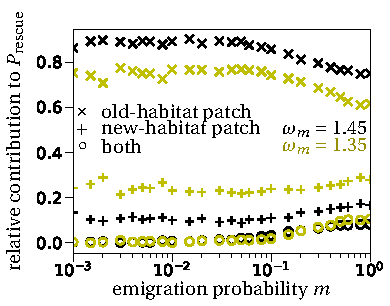
\includegraphics[width=\linewidth]{fig6a.pdf}
  		\caption{}
	\end{subfigure}%
    \begin{subfigure}{.5\textwidth}
 		 \centering
 		 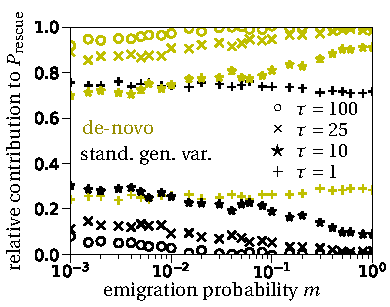
\includegraphics[width=\linewidth]{fig6b.pdf}
  		\caption{}
	\end{subfigure}
	\caption{\textbf{Habitat of origin of the rescue mutation and the impact of standing genetic variation.} \small (a) We compare the source of successful mutations under small (black) and large (yellow) fecundity differences in the old habitat. Decreasing the fecundity of the mutant results in more successful mutations emerging in new-habitat patches ($+$) when compared to the contribution from old-habitat patches ($\times$). We have chosen $\pi_m=\pi_w=0$. (b) For slower environmental degradation, i.e. $\tau=200$, the influence of standing genetic variation (sgv) on the probability of evolutionary rescue decreases. The simulations are done by letting the system evolve for $1,000$ generations before the first deterioration event happens. Parameters: $\pi_m=\pi_w=0$ in all scenarios and $\omega_m=1.45$. The relative contribution is then determined by $(P_{\text{rescue with sgv}}-P_{\text{rescue only de novo}})/P_{\text{rescue with sgv}}$.}
	\label{fig:sgv}
\end{figure}

So far, we have considered settings where evolutionary rescue is exclusively due to de novo mutations. To explore the role of standing genetic variation\footnote{\pete{or variance? is there a difference? why use one over the other?}}, we ran simulations \linelabel{R1-45}where we let the system evolve for $1,000$ generations before the first degradation event happened. Fig.~\ref{fig:sgv}(b) shows the relative contribution of de novo mutations and of standing genetic variation, i.e. mutations that appeared before the first degradation event happened. \linelabel{R2-39}\chg{For a successful rescue event due to standing genetic variation, mutants that were initially present (at time $t=0$) need to survive at least until sufficiently many patches have deteriorated that the probability of adaptation, $P_{\text{adapt}}$, becomes positive, compare to Fig.~\ref{fig:source_sink}(b,d) and Fig.~SX in the SI.} \linelabel{R1-46}\chg{Decreasing the value of $\tau$ reduces the time between two consecutive degradation events and the overall time-span of the entire environmental change. Therefore, the impact of standing genetic variation on the probability of evolutionary rescue increases for smaller values of $\tau$.}

Additionally, the relative contribution of standing genetic variation declines as the emigration rate $m$ increases. 
This holds because \linelabel{R1-49}\chg{the mutant is almost exclusively found in old-habitat patches if the frequency of these patches, $f_{\text{old}}$, and emigration rates $m$ are high} (see Fig.~SX in SI). Thus, mutants that existed prior to the first deterioration event are very unlikely to survive even for a rapidly changing environment. 

%%%%%%%%%%%%%%%%%%%%%%%%%%%%%%%%%%%%%%%%%%%%%%%%%%%%%%%%%%%%%%%%%%%
%%%%%%%%%%%%%%%%% DISCUSSION %%%%%%%%%%%%%%%%%%%%%%%%%%%%%%%%%%%%%%
%%%%%%%%%%%%%%%%%%%%%%%%%%%%%%%%%%%%%%%%%%%%%%%%%%%%%%%%%%%%%%%%%%%
\section*{Discussion}
%
% Brief summary
We have studied the probabilities of establishment, adaptation and evolutionary rescue under four non-\chg{uniform} dispersal schemes and compared them to \chg{unbiased} dispersal. Our analysis builds on the probability of establishment of a single mutant lineage in a heterogeneous environment with a fixed patch configuration. In line with previous results, we find that the probabilities of establishment, adaptation and evolutionary rescue can display up to three different phases when varying the dispersal rate $m$.
The different dispersal schemes, by changing the population dynamics, \chg{alter the parameter range of these regions.}\footnote{\francois{Unclear. Suggestion (not great but a bit better maybe): "The dispersal scheme determines the population dynamics and consequently the parameter regions corresponding to the three phases."}}
%broaden, tighten or shift these regions. 


\subsection*{Dispersal and adaptation}
% General comparison to other models and our resulting formula
Theoretical studies that investigated the effects of spatial subdivision on the adaptation of a population in a heterogeneous environment can be classified into two types. One type of models, classically analyzed in a population genetic context\francois{framework}, assumes constant population sizes in all patches, independent of their local habitat type and of dispersal strength. Results obtained in this framework show that larger dispersal rates tend to decrease the probability of successful establishment of a rare mutant favored in some part of the environment \citep[e.g.][]{garcia_1997}. This \st{inhibiting effect of dispersal on adaptation, also} \francois{effect} termed ``gene swamping'', is a result of an increase in absolute numbers of non-adapted individuals in the habitat where the rare mutant is beneficial \linelabel{R1-51}\chg{before reproduction and density regulation. This results in a lower mutant frequency \citep{lenormand_2002,tomasini_2018} and thus in lower reproductive success.} Additionally, for very high dispersal rates, the population homogenizes and individuals encounter an averaged environment. Therefore, the type with the largest overall growth rate, averaged over the environment, is favored.  \francois{In our model, gene swamping was rarely observed; the dominant effects were explained by the impact of dispersal on demography.} \footnote{\francois{Would consider shortening this paragraph which is not directly relevant. e.g. remove the sentence "this results in a lower mutant frequency...", but keep the references}}.

The second type of models explicitly takes into account demographic effects due to dispersal, often in the context of source-sink systems \citep{holt_1985,pulliam_1988}. 
Here, the effect of dispersal on adaptation depends on the growth rate differences of the mutant and the wild type in the two habitats \citep{kawecki_2000}. 
In accordance with this result \francois{these results}, we find that dispersal \francois{monotonically} increases the probability of adaptation if the mutant is just slightly less fit than the wild type in the old habitat %, $\omega_m / \omega_w= 0.99$
(Fig.~\ref{fig:vary_m_est}(c)). 
When the mutant's fecundity in old habitats, $\omega_m$, is smaller \francois{than what?}, establishment probabilities are non-monotonic with a local maximum at intermediate dispersal rates \francois{and increases at large dispersal rates thanks to relaxed competition} (Fig.~\ref{fig:vary_m_est}(a)). 
\st{However, if the mutant's disadvantage in old-habitat patches is even greater, i.e. $\omega_m$} \francois{When the fecundity of the mutant is even smaller, the local maximum remains but relaxed competition no longer occurs} \st{adaptation is also hindered for large dispersal rates. The establishment probability becomes hump-shaped } (cf. Fig.~S2 in SI). \footnote{\francois{I was confused by this paragraph so rephrased to make it more uniform and better describe the figures and the key differences}}.

\st{Hence, models with and without demographic change differ most at higher emigration rates. This corresponds to region (iii) in our analysis; we illustrate this point in} \francois{Compared to models with implicit demography, explicitly modelling the population dynamics causes relaxed competition that increases the probability of establishment at high dispersal rates }Fig.~S5 in SI, the non-demographic version of Fig.~\ref{fig:vary_m_est}. 

\francois{In figure S5, there does seem to have relaxed competition for curves orange and purple. So it's a bit confusing. Maybe remove those? Also I think a more balanced discussion of the three phases: initial rise thanks to exportation of mut in new habitats; decline due to back-migration; final increase due to relaxed competition, and which effect appears or not in the pop gen model, would be nice. Right now we focus a lot on relaxed competition.}


\subsection*{\linelabel{R1-52}\chg{Standing genetic variation} and evolutionary rescue}

\st{Besides the general structure of the probability of evolutionary rescue when varying the emigration probability $m$, }we also studied the effect \francois{contribution} of standing genetic variation on this quantity \francois{to evolutionary rescue}. 
We find that the contribution of standing genetic variation on the overall probability of evolutionary rescue increases with the speed of the environmental change, determined by $\tau$ (Fig.~\ref{fig:sgv}(b)). 
This observation has also been made in a quantitative genetics setting where the adaptive trait is continuous (and not discrete as in our model) \citep{matuszewski_2015}. Experimental results with \textit{Caenorhabditis elegans} indicate that under slow environmental change the impact of standing genetic variation is small \citep{guzella_2018}. This is because the evolution of the trait is driven by \textit{de novo} mutations with small effects. For a sudden or fast environmental change (small $\tau$), standing genetic variation becomes increasingly important for the probability of evolutionary rescue. These observations are in line with our findings in Fig.~\ref{fig:sgv}(b). %and other theoretical results obtained in this context \citep{matuszewski_2015}. 

\subsection*{The effect of \chg{biased} dispersal patterns on adaptation and evolutionary rescue}
The importance of considering dispersal schemes \chg{other than} \chg{unbiased} dispersal has been highlighted in several papers \citep{edelaar_2008,clobert_2009,edelaar_2012}. This has led to a number of simulation studies exploring the effect of various dispersal schemes onto \chg{(local)} adaptation %and niche width
\citep[e.g.][]{vuilleumier_2010,holt_2015,mortier_2018,pellerin_2018}. 

Two of these simulation studies examined the effects of matching habitat choice on adaptation \chg{in} a heterogeneous environment \citep{vuilleumier_2010,holt_2015}. Both investigations indicate that matching habitat choice increases the probability of adaptation when compared to \chg{unbiased} dispersal. 
This is in line with our findings: we predict that type-dependent habitat choice \chg{where each type favors patches they are relatively more fit in (Old-New),} generates higher probabilities of establishment \chg{(}and evolutionary rescue\chg{)} than \chg{unbiased} dispersal \chg{(0-0)} (Figs.~\ref{fig:vary_m_est}, \ref{fig:source_sink}, \ref{fig:rescue}). 

The dispersal schemes also slightly affect the origin of the successful mutant lineage, cf. SI, Fig.~S6. Population densities, especially in new-habitat patches, are altered when compared to the \chg{unbiased} dispersal scheme.\footnote{\pete{This paragraph could be dropped in line with a comment of a reviewer.} \francois{agree to drop it}}

To conclude, the effects of dispersal schemes are two-fold. By changing population densities in both habitat types, the dispersal schemes \chg{alter} the growth rate of the mutant in old-habitat patches. 
This is the primary reason for the ranking of the dispersal schemes. In addition, they also affect the number of mutations arising in either habitat type. This has a minor effect on the probability of evolutionary rescue for the explored parameter range but is relevant when studying the origin of the successful mutant\florence{mutation} lineage \chg{(see also SI, Fig.~S6)}. \francois{As the genetic background may vary across patches, the origin of a successful mutation will also affect which neutral and deleterious mutations will hitchhike with it}. \linelabel{R1-54}\chg{The origin of a successful mutant is of special interest once multiple loci are considered\francois{. Rescue by a single mutant implies} \st{which might promote} neutral (or even deleterious) hitchhiking effects. Similarly, in the case of polygenic rescue or under recombination \citep[e.g.][]{uecker_2015}, the origin of a mutant is likely to affect its success.}\florence{[mention genetic background]}    

% \subsection*{Evolutionary consequences of habitat choice}
% The interplay of local adaptation and habitat choice has interested evolutionary ecologists for several decades, see for example \citet{rosenzweig_1981} for one of the first references. 
% Our analysis shows that absolute habitat choice lowers the probability of establishment when compared to random dispersal; see blue lines in Fig.~\ref{fig:vary_m_est}. 
% This indicates that habitat choice protects a population against locally deleterious mutations, that are potentially favorable elsewhere, if the mutant has the same dispersal pattern as the wild type, i.e. $\pi_m=\pi_w>0$. A similar observation, protection of the already established type, was made in \citet{ravigne_2009} where a co-evolutionary model of a habitat choice trait and a local adaptation trait is implemented. 
% %This is achieved by maintaining a large local density in old-habitat patches which increases the local selection strength. Therefore, fecundity differences between the mutant and the wild type have a strong impact on the composition of the next generation. 

% Moreover, \citet{ravigne_2009} find that habitat choice can actually evolve and lead to evolutionary branching, i.e. the coexistence of two specialist types with their own habitat preferences (our relative habitat choice dispersal scheme). 
% %In a scenario where habitat choice and adaptation to the habitat are two independent traits, the adaptive mutant will share the habitat preference of the wild type at its emergence. For strong habitat preferences (large $\pi_w$) this can result in new patches remaining empty. This observation was also made in \citet{ravigne_2009}\footnote{\florence{Shorten; just say habitat choice could evolve (Ravigne 2009)}} -- even though in a different model not exhibiting source-sink dynamics and under a different regulation scheme. 
% %In that study, the authors analyzed the co-evolution of a habitat choice trait and a local adaptation trait. 
% %Translating their results (from their `model~1' that is closest to our life cycle) into our framework they find that relative habitat choice (orange) enhances evolutionary branching, i.e. the coexistence of two specialist types with their own habitat preferences. In contrast, absolute habitat choice protects the already established type (or at best creates a generalist type for the whole environment). 
% In line with this, our results show that in parameter regions where relative habitat choice yields higher probabilities for establishment than random dispersal, if a mutant is able to quickly evolve its own habitat preference as it does in \citet{ravigne_2009}, it has an increased chance of establishing in the meta-population. This is in agreement with recent experimental findings in the ciliate \textit{T. thermophila} \citep{jacob_2017}. Even though we do not explicitly consider speciation and the evolution of genetic polymorphisms, our results may suggest that type-dependent matching habitat choice enhances phenotypic divergence, if we use the probability of adaptation as a proxy for invasion probability. The probability of adaptation for relative habitat choice (orange) is higher than for absolute habitat choice (blue) or random dispersal (black), Fig.~\ref{fig:source_sink}. This idea has already been promoted in other theoretical and experimental studies \citep[e.g.][]{rosenzweig_1987,rice_1990,ravigne_2009,berner_2015,jacob_2018}.

\subsection*{Generality of our theoretical analysis and future directions}
Our mathematical results apply in the case where the mutant offspring numbers can be written in the form ``migration times reproduction (and potential regulation)'' with rates that are constant in time (\linelabel{R1-58-1}\chg{or as in case of evolutionary rescue, constant between two deterioration events}; see the mean reproduction matrix in eq.~\eqref{eq:mean_repro}). Biologically, this means that the resident population is stationary and the mutant is either at low numbers or unaffected by its own density. Furthermore, for our approximation in eq. \eqref{eq:estab_approx} to generate accurate predictions, it is essential that growth rate differences between the wild type and the mutant are weak and dispersal is low. Formally, just two of these parameters need to be small -- see also the corresponding discussion in \citet{tomasini_2018}. 

Since we summarize the population dynamics in our parameters of the reproduction matrix, the approach taken here is quite general and can account for various dispersal schemes and local \chg{type-dependent} population dynamics, \linelabel{AE-3-1}\chg{i.e. different reproduction and competitive parameters.} However, it cannot account for \chg{type-dependent carrying capacities, explicit spatial structure %as for example the stepping stone model. It also cannot account for 
or \st{time-inhomogeneous} \francois{rapidly changing} environments.} \linelabel{R1-58-2} The \chg{latter} is the reason for our \chg{poor}\footnote{\pete{any better word here?}} approximation in the context of evolutionary rescue (Fig.~\ref{fig:rescue})\footnote{\francois{I would remove this sentence}}. Additionally, in order to obtain analytical solutions, it is important that the stationary population sizes of the wild type have an accessible solution. This is not the case if we consider non-linear emigration rates that depend on habitat choice like those incorporated in some simulation studies \citep[e.g][]{holt_2015,mortier_2018}.  

In contrast, it \chg{is} possible to \chg{implement} a cost of dispersal \chg{or} a different life cycle. In particular, the variation of the life cycle could yield \chg{distinct} results regarding adaptation \citep{holt_2015} and, more generally, in the context of the evolution of dispersal \citep{massol_2015}. \\

In conclusion, we studied the effect of dispersal and different dispersal schemes on the probability of establishment, adaptation and evolutionary rescue of a mutant under divergent selection in a subdivided population. Our quantitative approach disentangles the interaction of dispersal and adaptation. We recover previous results on adaptation and provide a general framework for studying evolutionary dynamics of a subdivided population in heterogeneous environments \chg{in discrete time}. This unifying approach allows us to identify the forces responsible for the different predictions obtained in the population genetics literature and under source-sink dynamics, respectively. We find that including population demography significantly alters the results for high dispersal rates. For constant population sizes, high dispersal rates have a negative effect on establishment, while with explicit demography the effect is largely positive. The latter is a result of relaxed competition in old-habitat patches. Most importantly, we extend the existing literature by comparing different dispersal schemes and studying their effects on adaptation and evolutionary rescue. Our results indicate that habitat choice does not necessarily result in an increased adaptive potential and might even hinder successful establishment of a mutant population that would avoid population extinction. \linelabel{R1-60} %Negative density-dependent dispersal always increases the probability of adaptation and evolutionary rescue. 
These results show that non-\chg{uniform} dispersal patterns can have a strong influence on population survival and adaptation in a heterogeneous environment. 

\subsection*{Acknowledgements}
PC and FD received funding from the Agence Nationale de la Recherche (ANR-14-ACHN-0003 to FD). HU appreciates funding from the Max Planck Society. We are grateful to the INRA MIGALE Bioinformatics Facility (MIGALE, INRA, 2018. Migale Bioinformatics Facility, doi: 10.15454/1.5572390655343293E12) for providing computational resources. Additionally, we thank J\'{e}r\^{o}me Mathieu for highlighting the connection of the `New-Old dispersal scheme' to the ecological trap literature, and Staffan Jacob and Pim Edelaar for fruitful discussion concerning the biological motivation of the dispersal schemes. 

\bibliographystyle{plainnat}
\bibliography{dispersal.bib}

\end{document}